\chapter{Energetic Patterns of Cyclones in the Southwestern Atlantic}\label{ch:energetic_patterns}


Chapter \ref{ch:energetics} investigated the LEC climatology for the cyclones with genesis in the South American sector. Although the mean behavior across all systems was discussed, the results exhibited high variability, which hindered a deeper analysis of patterns that deviated from the norm. This chapter will employ clustering analysis to determine patterns in the LEC — energy patterns — related to eddy development, so this variability can be further assessed. 

\section{Lorenz Phase Space and Energy Patterns}\label{sec:lps}

\subsection{Introducing the Lorenz Phase Space}

The first step in constructing the energy patterns (EP) involves devising a visualization that could facilitate the understanding of the environmental energetics related to cyclonic systems. As demonstrated in Chapter \ref{ch:energetics}, the usual LEC visualization (where arrows representing energy fluxes connect the distinct energy terms) is a powerful tool for understanding the atmospheric dynamics associated with atmospheric systems and their evolution. However, it is not practical for large datasets and considering multiple phases denoting the systems' evolution over time, as is the case here. Therefore, the goal of this section is to devise a new visualization tool that simplifies this process while maintaining the focus on displaying the dynamics related to eddy development, i.e., related to their Efficient and Final Causes (Sections \ref{efficient_causes} and \ref{final_causes}).

Figures \ref{fig:lps_1_reg1} and \ref{fig:lps_2_reg1} contain Phase Diagrams, inspired by the Cyclone Phase Space created by \citet{hart2003cyclone}, in which distinct sets of the LEC terms are represented. These representations are called Lorenz Phase Space (LPS) diagrams. As mentioned, these diagrams focus on the mechanisms related to eddy growth. Evidently, there is a trade-off between representing as many terms as possible but keeping some degree of simplicity, while still providing an intuitive visualization.

\begin{figure}[!htbp]
\centering
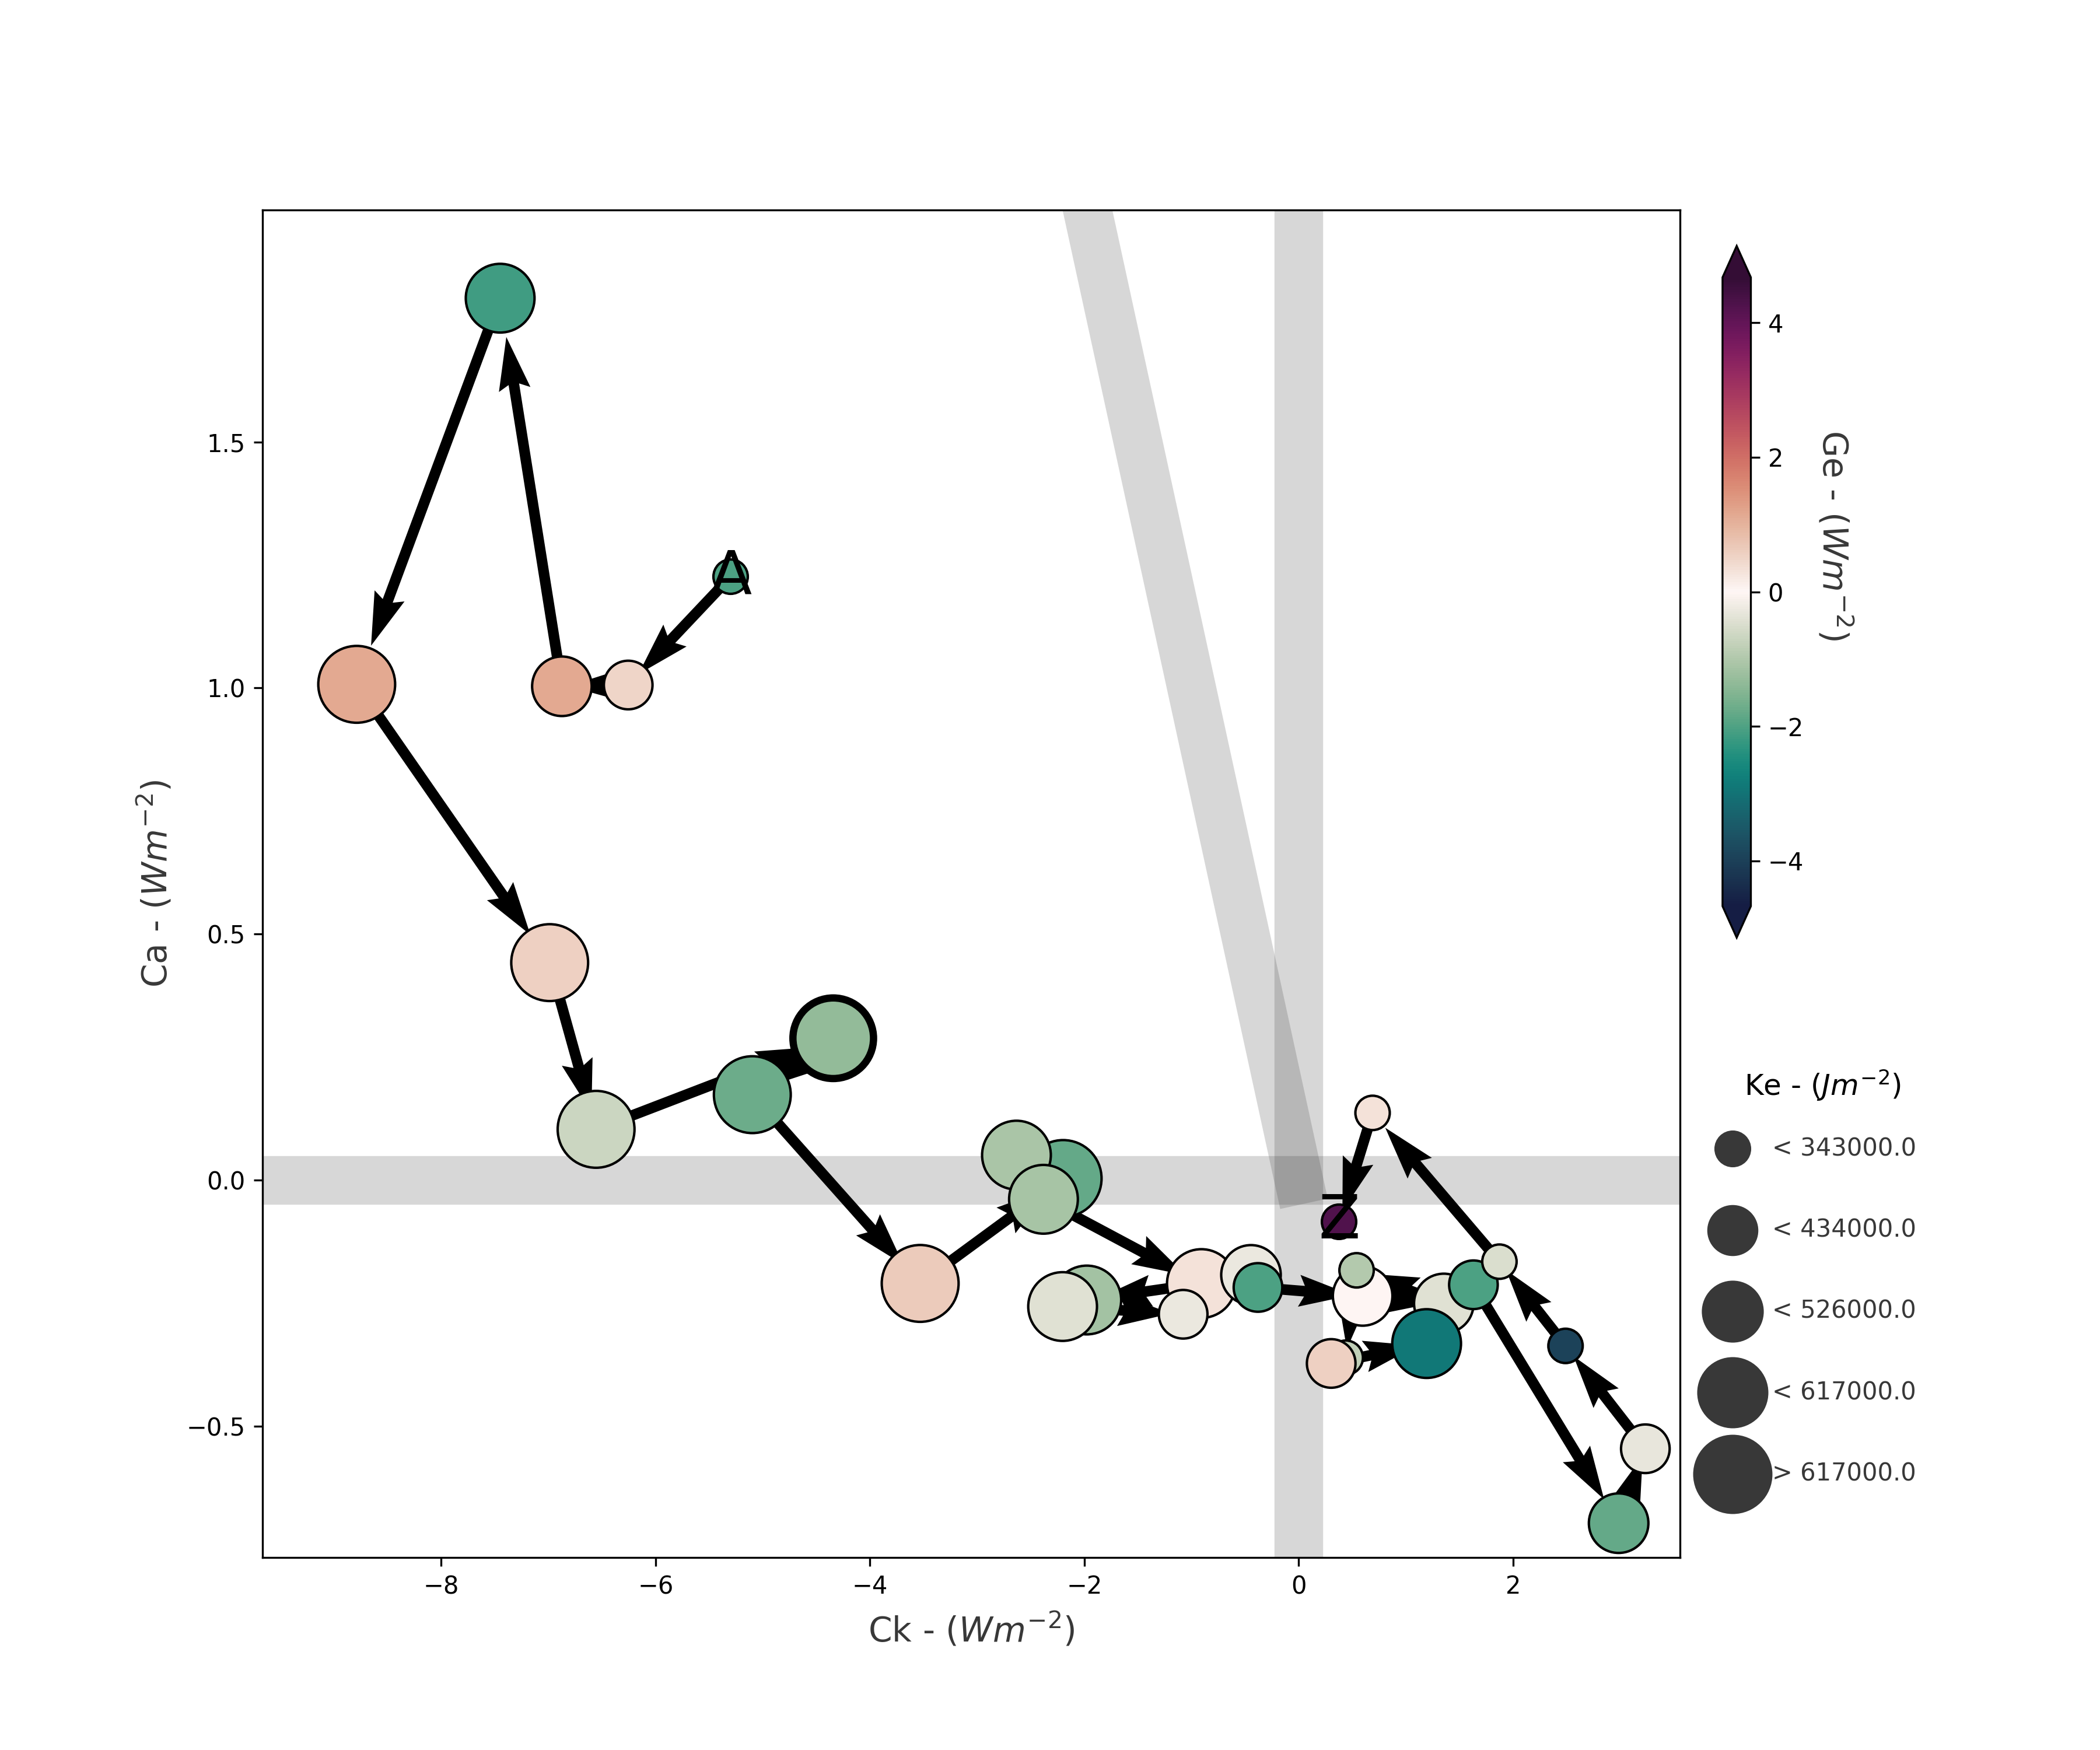
\includegraphics[width=\textwidth]{figs_6/lps-mixed_Reg1-Representative_NCEP-R2_fixed.png}
\caption[LPS 1 - "Reg1" Cyclone]{Lorenz Phase Space (LPS) diagram 1 for "Reg1" cyclone \citep{dias2011energy}. The x-axis represents the barotropic conversion term ($C_K$), which indicates the conversion from zonal to eddy kinetic energy, while the y-axis shows the baroclinic conversion term ($C_A$). The color shading denotes the generation of eddy potential energy ($G_E$), with warmer colors indicating higher convective activity and cooler colors representing lower activity. The size of the circles correlates with the system intensity, measured by $K_E$. The letters "A" and "Z" mark the system's initial and final positions, respectively. The point where the system reaches its peak intensity is highlighted by a thick circle border.}
\label{fig:lps_1_reg1}
\end{figure}

Figure \ref{fig:lps_1_reg1} displays the LPS representing the main terms related to dynamical instabilities in the atmosphere. The x-axis represents the barotropic conversion term ($C_K$), the y-axis the baroclinic conversion term ($C_A$), while the color shading represents the convective activity ($G_E$) and the circle sizes represent the system intensity ($K_E$). There is also an "A" and a "Z" representing the system's initial and final positions, and the moment where the system is most intense is marked by a thick circle border. Meanwhile, Figure \ref{fig:lps_2_reg1} illustrates the LPS related to imports of Eddy Energy. This diagram is similar to Figure \ref{fig:lps_1_reg1}, but here the x-axis represents importation and exportation of eddy APE across the system boundaries ($BA_E$), while the y-axis shows the importation and exportation of eddy kinetic energy across the system boundaries ($BK_E$). 

The choice for using the $C_A$ term in the LPS diagram (Figure \ref{fig:lps_1_reg1}) is justified by its high correlation with the $C_E$ term (Appendix \ref{ap04}). Thus, when positive conversions from $A_Z$ to $A_E$ occur, there is a high probability that conversions from $A_E$ to $K_E$ are also happening, indicating an active baroclinic chain. Additionally, since the second LPS diagram (Figure \ref{fig:lps_2_reg1}) represents the imports of $A_E$ and both LPS diagrams indicate $G_E$, the $C_E$ signal can be inferred. Meanwhile, the $K_E$ was chosen to represent the system's intensity because it generally increases from genesis to the mature phase and decreases during the decay phase (Section \ref{sec:climatology_phases}). It also correlates well with central relative vorticity at 850 hPa (Appendix \ref{ap04}).

On Figures \ref{fig:lps_1_reg1} and \ref{fig:lps_2_reg1}, the energetics of the "Reg1" system from \citet{dias2011energy} are analyzed using the LPS diagrams. Here, for comparison with the original results, the same computational procedure as from \citet{dias2011energy} is used (Eulerian Framework), for the same domain, as well as the same dataset (NCEP-R2 reanalysis). The computational domain and time series for energy and conversion terms are presented in Appendix \ref{ap05}. The only difference is that here $G_E$ is used instead of $RG_E$, in order to allow for a physical interpretation of this term's contributions.

Using the LPS diagrams, one can easily identify the dynamical mechanisms inciting eddy development associated to the cyclone system. For instance, Figure \ref{fig:lps_1_reg1} indicates that during the system's early life stages, baroclinic and barotropic conversions provided support for its development, as well as contributions from convective processes (evidenced by $G_E$). As the system's life progresses, the importance of baroclinic conversions and convective processes diminishes, with both terms becoming negative and the eddy being sustained only by barotropic conversions. During later periods, $G_E$ is negative, and the eddy is feeding the zonal circulation, as well as $K_E$ being converted to $A_E$. 

Negative $G_E$ indicates APE destruction, (i.e., cooling where temperature perturbation is positive and warming where temperature perturbation is negative). Cooling is associated to either evaporative cooling or long wave radiative energy loss. Warming is either associated to latent/fusion heating or short wave radiantive energy loss. Sensible heating near the surface can be positive or negative, depending on the temperature difference between the surface and the air.

Meanwhile, Figure \ref{fig:lps_2_reg1} shows that in the initial development stages, there were exports of both $A_E$ and $K_E$ outside the domain, but as the system developed, both boundary terms reverted to imports of energy, with higher magnitudes than the conversion terms displayed in Figure \ref{fig:lps_1_reg1}. Also, in later development stages, as the combined magnitudes of $C_A$ and $BA_E$ were lower than $G_E$, it can be inferred that $C_E < 0$, so the eddy-driven thermal circulation had stopped, and the equator-to-pole temperature gradients were being reestablished.


\begin{figure}[!htbp]
\centering
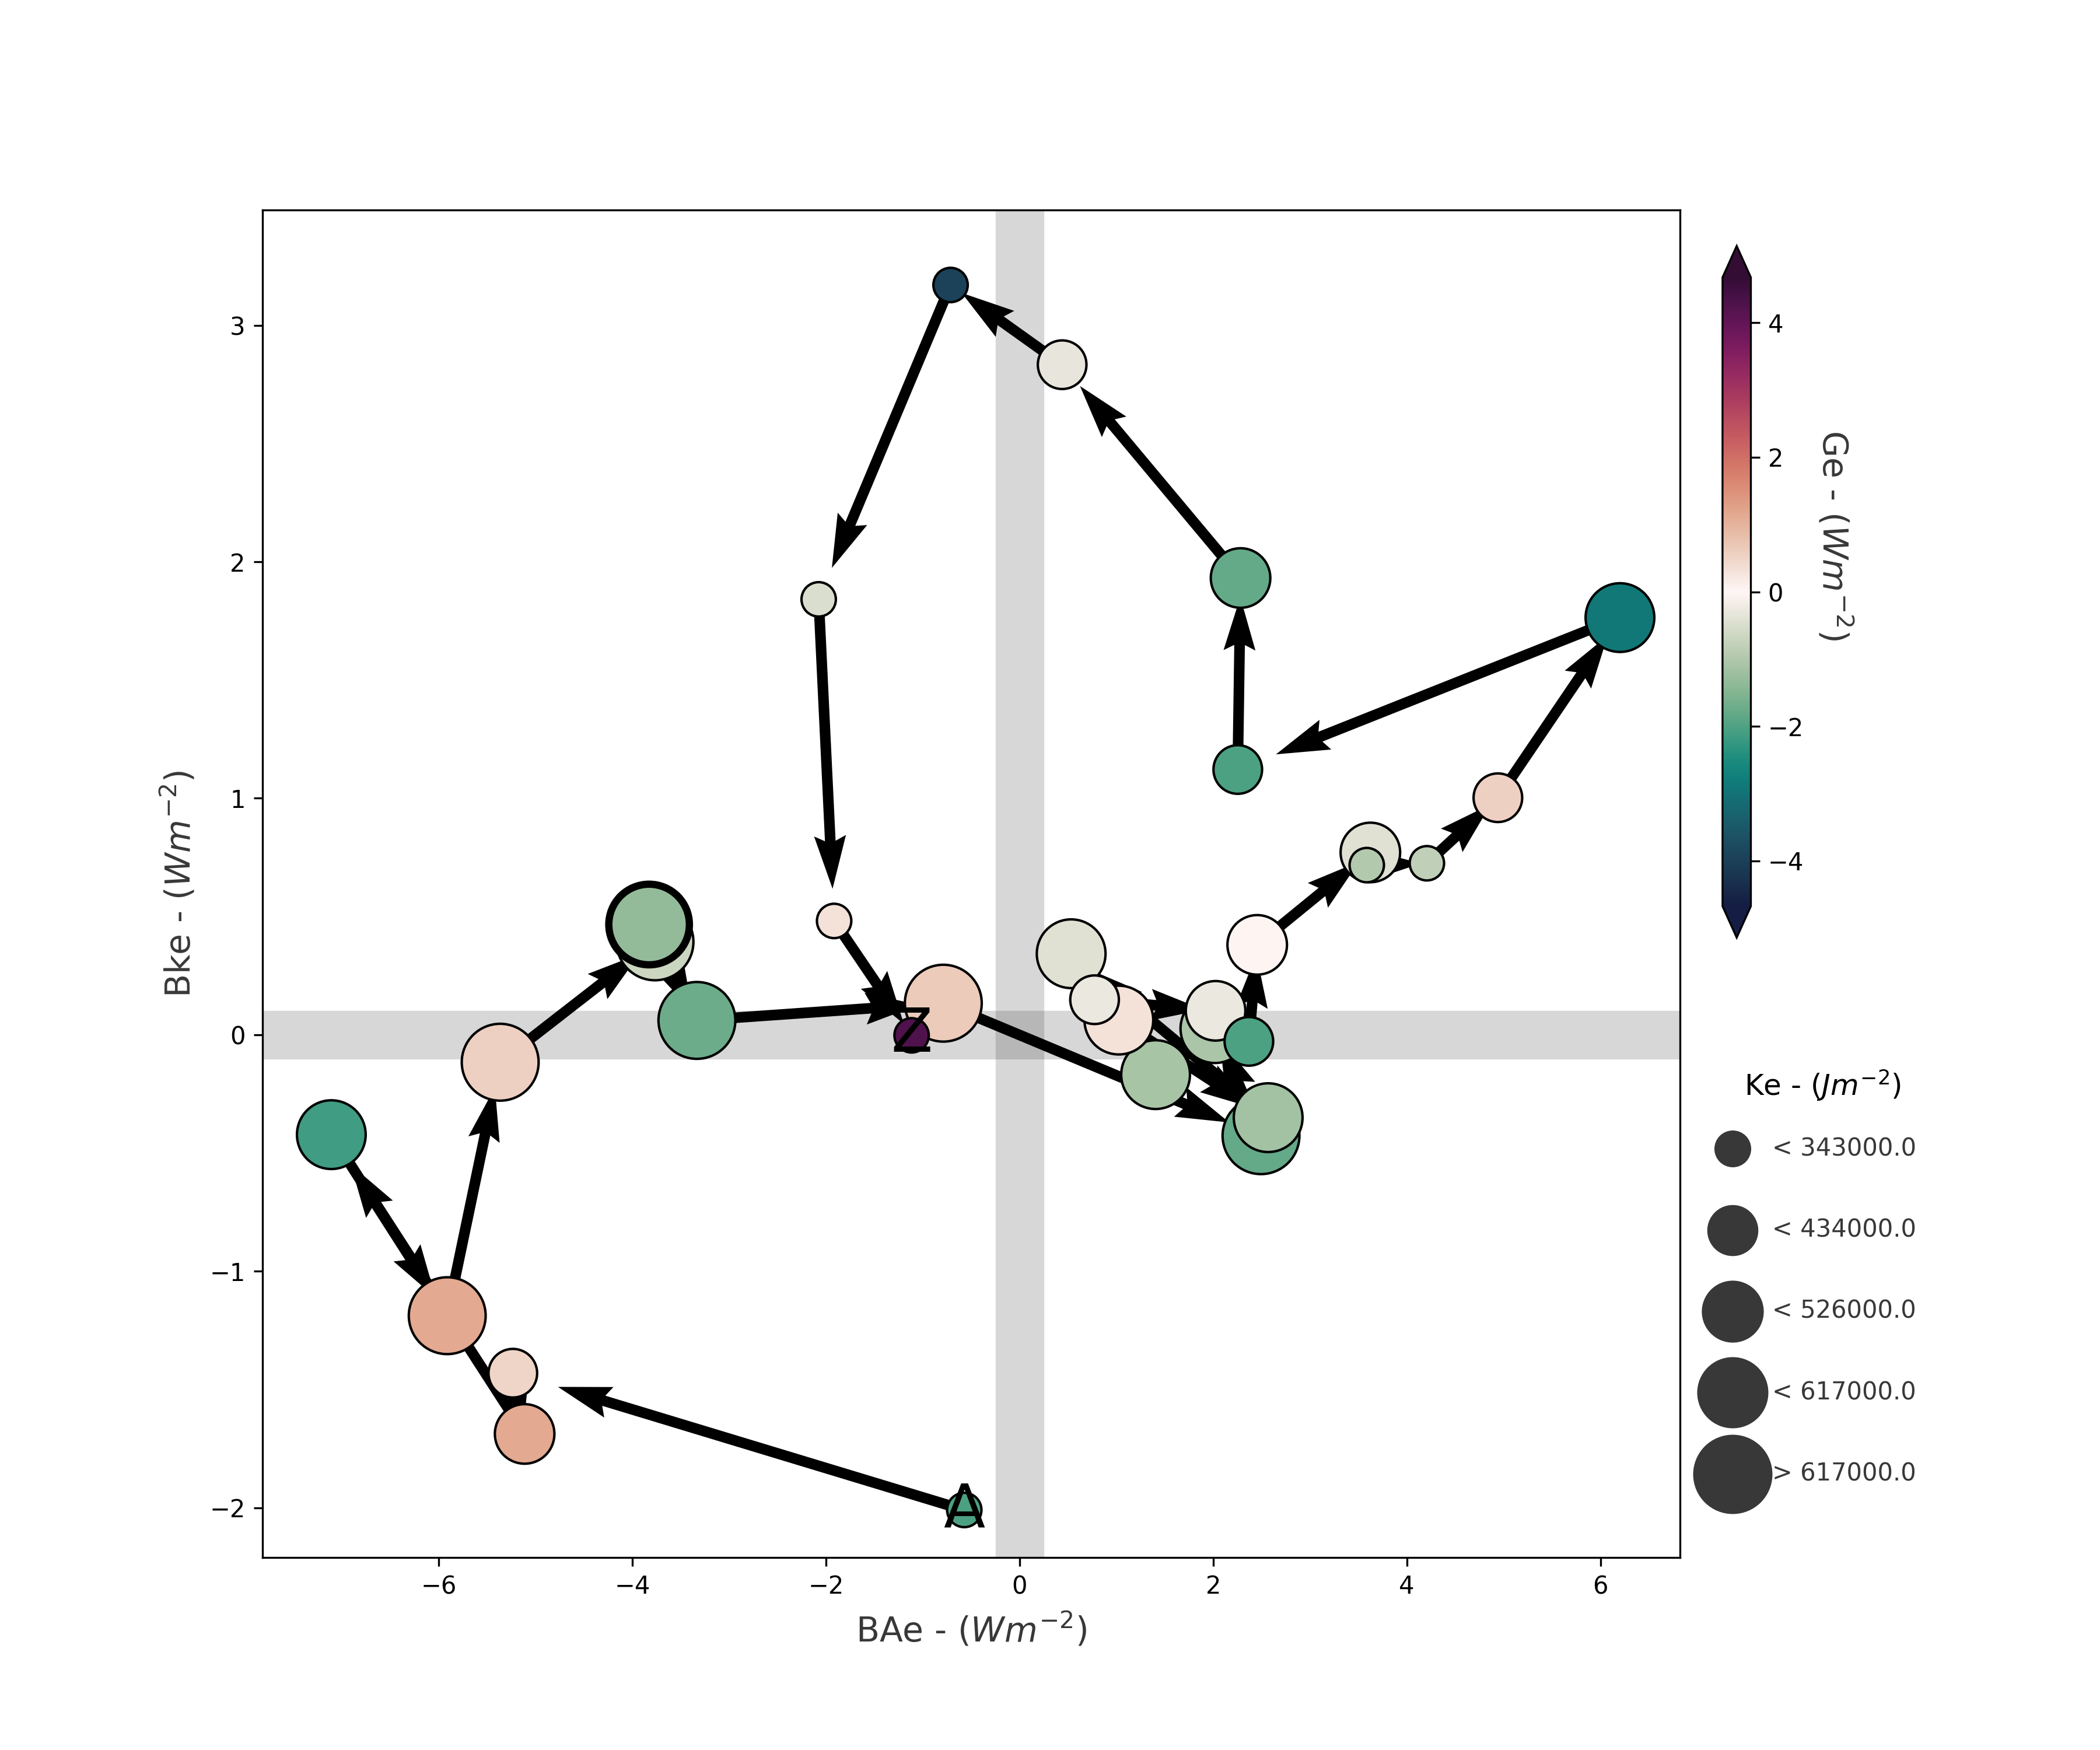
\includegraphics[width=\textwidth]{figs_6/lps-import_Reg1-Representative_NCEP-R2_fixed.png}
\caption[LPS 2 - "Reg1" Cyclone]{Lorenz Phase Space (LPS) diagram 2 for "Reg1" cyclone \citep{dias2011energy}. The x-axis represents importation and exportation of eddy APE across the system boundaries ($BA_E$), while the y-axis shows the importation and exportation of eddy kinetic energy across the system boundaries ($BK_E$). The color shading denotes the generation of eddy potential energy ($G_E$), with warmer colors indicating higher convective activity and cooler colors representing lower activity. The size of the circles correlates with the system intensity, measured by $K_E$. The letters "A" and "Z" mark the system's initial and final positions, respectively. The point where the system reaches its peak intensity is highlighted by a thick circle border.}
\label{fig:lps_2_reg1}
\end{figure}


% (EXPLAINING MIXED LPS) This diagram can be split into four quadrants, each representing distinct dynamical processes. In the top-right quadrant, both $C_A$ and $C_K$ are positive, so while $A_E$ is providing energy to $K_E$, $K_E$ is providing energy to the mean zonal circulation ($K_Z$). It can be said that while the eddy is gaining APE from the mean flow, it is also providing kinetic energy to it. In the bottom-left quadrant, both conversion terms are negative, so while the eddy is providing APE to the mean flow, it is also receiving kinetic energy from it. The top-left quadrant represents both previous processes happening simultaneously, with the eddy receiving both APE and kinetic energy from the mean flow, thus relating to both instability processes. Lastly, in the bottom-right quadrant, the eddy is providing both APE and kinetic energy to the mean flow, feeding the local atmospheric circulation.

\subsection{Energetic Patterns for All Life Cycle Configurations}\label{sec:energy_patterns}

The LPS diagrams containing all systems for the SESA region for the 1979-2020 period can be found in Appendix \ref{ap:06}. Due to the large amount of data and the presence of outliers, it is not possible to discern the relative importance of the LEC terms for smaller groups of systems precisely. Therefore, the K-means algorithm is employed to group the energy cycles into distinct representative clusters.

The first attempt at clustering all cyclones' energetics in the dataset is performed for all major lifecycle configurations, presented in Chapter \ref{ch:life_cycle} (Figure \ref{fig:filtered_lifecycle_configurations}b). Thus, the LEC terms were averaged for each life cycle phase, and each life cycle configuration was clustered independently. For all life cycle configurations analyzed, the elbow method returned an ideal number of clusters as 3, as represented in Figure \ref{fig:elbow_method_plot}. This figure corresponds to the "Incipient, Intensification, Mature, Decay" life cycle configuration, but the plots for each configuration were nearly identical.

\begin{figure}[!htbp]
\centering
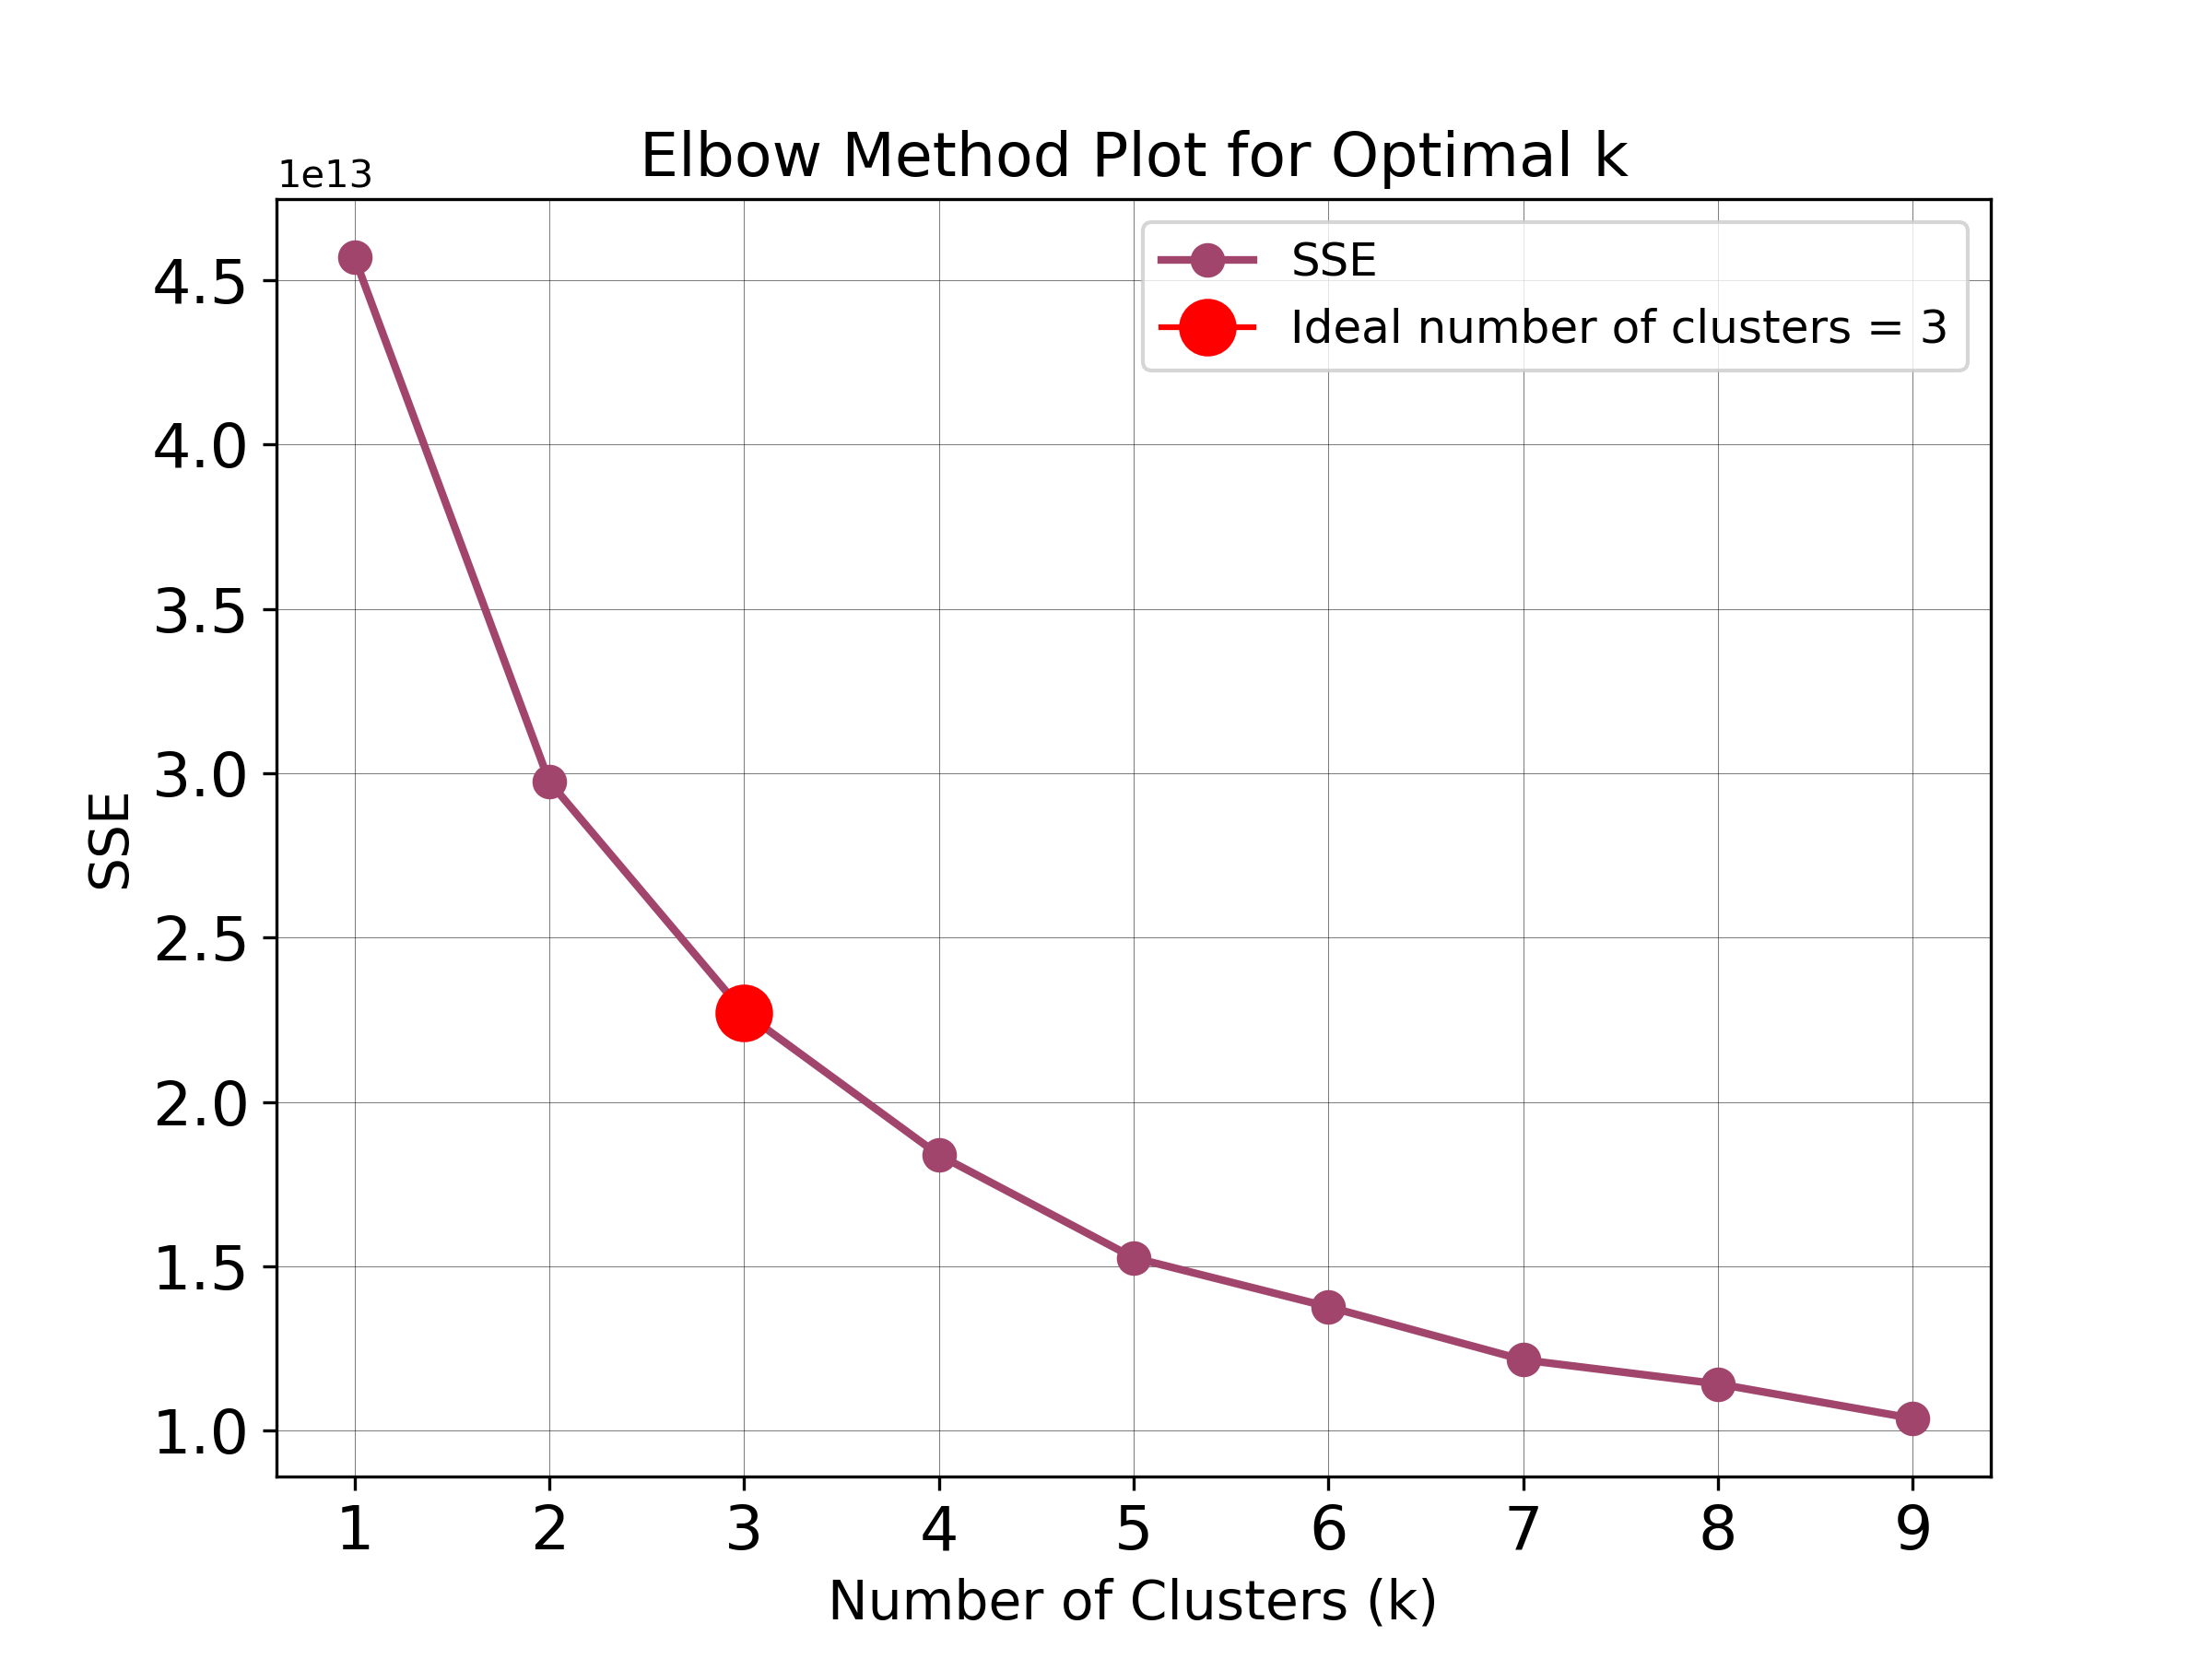
\includegraphics[width=0.8\textwidth]{figs_6/elbow_method_plot.png}
\caption[Elbow Method]{Elbow method plot for determining the optimal number of clusters. The x-axis represents the number of clusters (k), while the y-axis indicates the Sum of Squared Errors (SSE). The purple line shows the SSE for each k value. The red dot highlights the optimal number of clusters (k=3), where the SSE begins to decrease at a slower rate, forming an "elbow." This point suggests that three clusters provide a good balance between minimizing variance within clusters and model simplicity.}
\label{fig:elbow_method_plot}
\end{figure}

Figures \ref{fig:lps_mixed_clusters_all_life_cycles} and \ref{fig:lps_imports_all_systems_zoom} present the LPS diagrams for the centroids of the three clusters for each life cycle configuration. On these diagrams, each circle represents the energetics corresponding to a distinct life cycle phase, initiating on the incipient phase (A) and ending of either the first or second decay phases (Z). The centroids, which represent the mean positions of all data points within a cluster, serve as representative profiles of the LEC terms for the respective clusters. These centroids are not actual data points from the dataset but synthetic constructs that encapsulate the average characteristics of the LEC terms within each cluster. Consequently, they provide a generalized yet insightful depiction of the typical energy dynamics observed in the cyclonic systems classified within each cluster. This clustering approach allows us to identify and characterize distinct energetic patterns (EPs), facilitating a deeper understanding of the underlying physical processes driving the variability in cyclonic energetics.

\begin{figure}[!htbp]
\centering
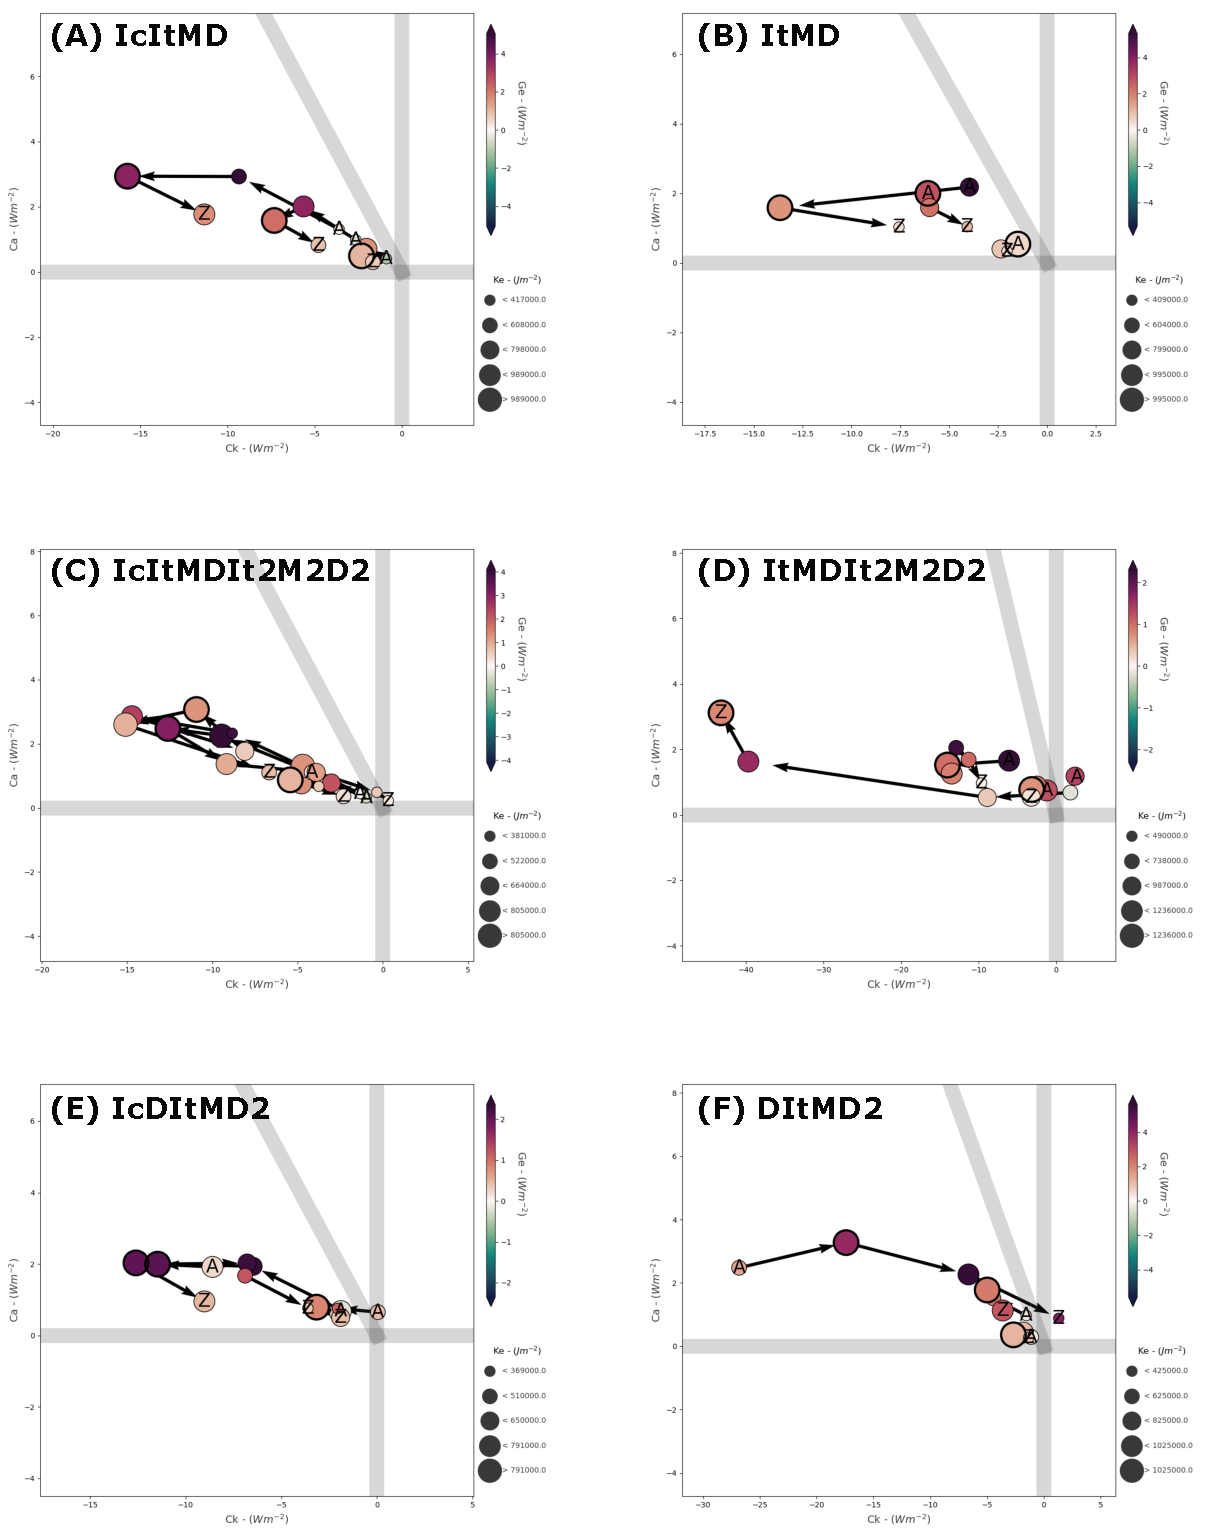
\includegraphics[width=\textwidth]{figs_6/lps_mixed_clusters_all_life_cycles.pdf}
\caption[LPS 1 - Clusters - All Life Cycle Configurations]{Lorenz Phase Space (LPS) diagram 1 for all main life cycle configurations (Figure \ref{fig:filtered_lifecycle_configurations}b). "Ic", "It", "M," and "D" denote incipient, intensification, mature, and decay phases, respectively, while a "2" is used to denote their second occurrence within the same life cycle configuration.}
\label{fig:lps_mixed_clusters_all_life_cycles}
\end{figure}

The LPS 1 diagram (Figure \ref{fig:lps_mixed_clusters_all_life_cycles}) indicates similar patterns emerging for all life cycle configurations, with systems often initiating in low energy states. As they intensify, both baroclinic and barotropic conversions, as well as convective activity, become more vigorous. Meanwhile, when the systems are decaying, they tend to revert back to lower energy states. The EPs within the same life cycle group usually differentiate from each other by the magnitude of the conversion and generation terms in each phase. It is notable that $C_K$ is usually higher than the other forms of energy, while $G_E$ and $C_A$ present comparable magnitudes. This reinforces the conclusion in Chapter \ref{ch:energetics} that barotropic conversions are one of the main mechanisms driving cyclone development in the SESA region.

There are some exceptions to the overall energetic development pattern described above. For example, for the "intensification, mature, decay" configuration (Figure \ref{fig:lps_mixed_clusters_all_life_cycles}b), there is an EP which already initiates with relatively high conversion levels and convective activity, decreasing in later stages, while another pattern starts with the highest $G_E$ values for this life cycle configuration EPs. Enhanced convective activity in the initial stages can also be noted for the configuration where "intensification, mature, decay" repeats twice (Figure \ref{fig:lps_mixed_clusters_all_life_cycles}d). This enhancement of energy conversion and/or generation is expected for these configurations, as they lack an incipient stage. In the Cyclophaser program, the incipient stage is not detected if the system's life starts with a relatively steep increase in relative vorticity (becoming more negative, i.e., becoming more intense) and if this process is fast enough that the duration criteria for phase detection are not met. Therefore, the LPS diagram 1 suggests that for these cases, the enhanced conversions/generation in earlier life periods are responsible for an abrupt intensification phase and the lack of an incipient phase.

Furthermore, another exception can be found in systems presenting an early decay phase (Figure \ref{fig:lps_mixed_clusters_all_life_cycles}f). In this case, one EP starts with a high energy state and then reverts to lower energy states as the system evolves. This EP, which roughly corresponds to only 3\% of the variability for this life cycle, representing less than 3\% of the cyclones in the total dataset, is composed of only four systems. Further examination revealed that this high energy state is linked to an outlier within this EP, while the other systems start in lower energy states (Appendix \ref{ap:07}). Although further examination of the dynamics related to this outlier is of interest, it is beyond the scope of the current study.


The LPS 2 diagram (Figure \ref{fig:lps_imports_all_systems_zoom}) presents a more heterogeneous behavior, although an overall pattern can still be observed. Systems often initiate with imports of $A_E$, which decrease as they develop. During the intensification phase, imports of $K_E$ increase, diminish in the mature phase, and revert to exports of $K_E$ during decay. As with LPS 1, the clusters for each life cycle configuration tend to differentiate from each other by the magnitude of the boundary and generation terms in each phase. The magnitude of the boundary terms is often comparable to $C_A$ and $G_E$, and for some EPs at specific phases, they present higher values, comparable to $C_K$ values. Similarly, as noted for LPS 1, the EPs lacking an incipient stage often initiate in higher energy states, reinforcing the argument that rapid intensification in these cases is related to an enhanced energy cycle. Meanwhile, the outlier for the life cycle configuration with an early decay can still be noted (Figure \ref{fig:lps_imports_all_systems_zoom}f).

\begin{figure}[!htbp]
\centering
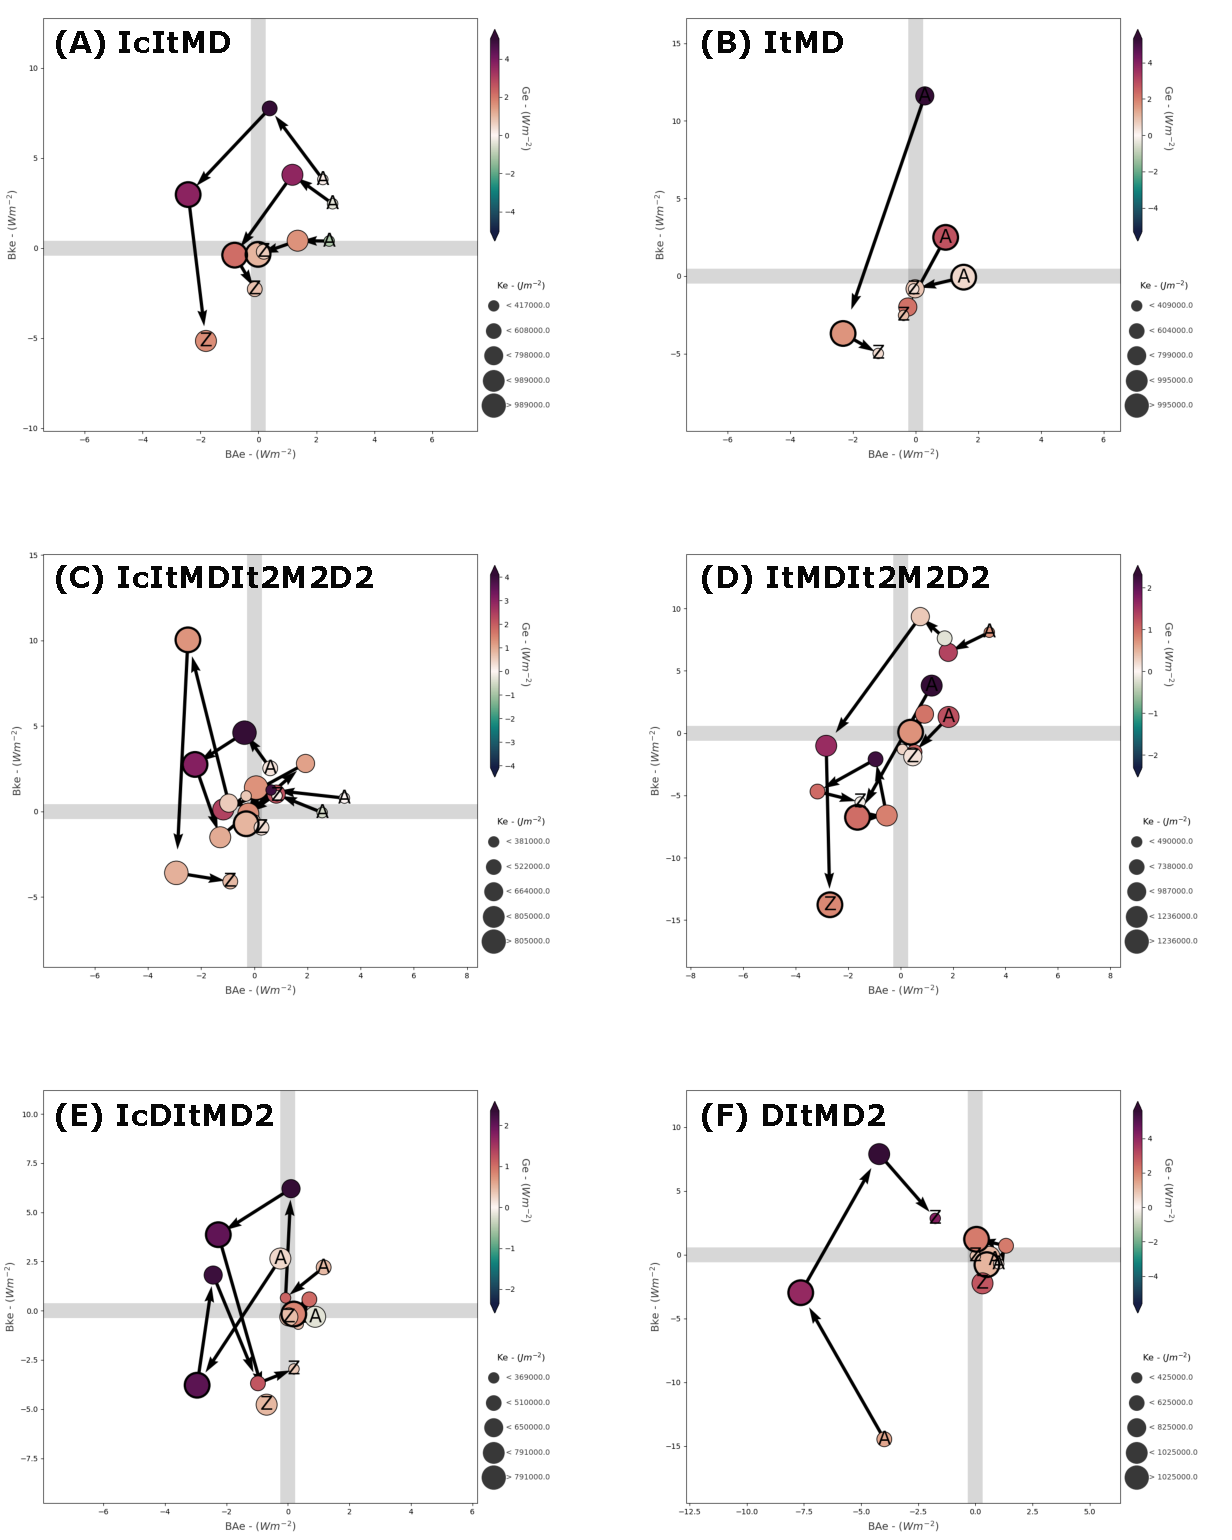
\includegraphics[width=\textwidth]{figs_6/lps_imports_clusters_all_life_cycles.pdf}
\caption[LPS 2 - Clusters - All Life Cycle Configurations]{Lorenz Phase Space (LPS) diagram 2 for all main life cycle configurations (Figure \ref{fig:filtered_lifecycle_configurations}b). "Ic", "It", "M," and "D" denote incipient, intensification, mature, and decay phases, respectively, while a "2" is used to denote their second occurrence within the same life cycle configuration.}
\label{fig:lps_imports_all_systems_zoom}
\end{figure}

Given that the behavior presented by the EPs shows low variability among distinct life cycle configurations, the next sections will focus on the EPs for the "incipient, intensification, mature, decay" configuration for simplicity (Figure \ref{fig:lps_mixed_clusters_all_life_cycles}a). This choice is also justified by the prevalence of this life cycle configuration within the dataset, representing nearly 60\% of all systems (Figure \ref{fig:filtered_lifecycle_configurations}b). This approach allows for more detailed analysis while maintaining the potential for generalizing the results.

\subsection{Energetic Patterns - Seasonality and Spatial Variability}\label{sec:energy_patterns_season_region}

While Section \ref{sec:energy_patterns} focused on the differences of the EPs among the distinct life cycle configurations, the present section will investigate their seasonality and spatial variability. As previously discussed, the focus will be on the EPs for the "incipient, intensification, mature, decay" life cycle configuration. The spatial and seasonal variability is assessed by employing the clustering technique for the distinct seasons and genesis regions in the Southwestern Atlantic region: ARG, LA-PLATA, and SE-BR, as delineated in Chapter \ref{ch:life_cycle}. For this analysis, the K-means algorithm was initialized for each region and season separately. As in Chapter \ref{ch:life_cycle}, only austral summer (DJF) and winter (JJA) are assessed.

Figure \ref{fig:lps_mixed_clusters_IcItDM_seasons_regions} presents the LPS 1 diagram for the EPs related to each region, for JJA and DJF. Notably, for each season-region group, the elbow method detected an optimal number of clusters as three, similarly to the EPs for all systems. It can be seen that the overall behavior is preserved across the distinct seasons and regions: the systems often initiate in lower energy states, and as they develop, the energy conversions, as well as convective activity, become more intense. Within each group, each distinct EP represents an overall higher energy state: one EP presents more neutrality for $C_A$, $C_K$, and $G_E$ for all life phases, while the second and third EP progressively present higher conversions and often higher generation of $A_E$.


\begin{figure}[!htbp]
\centering
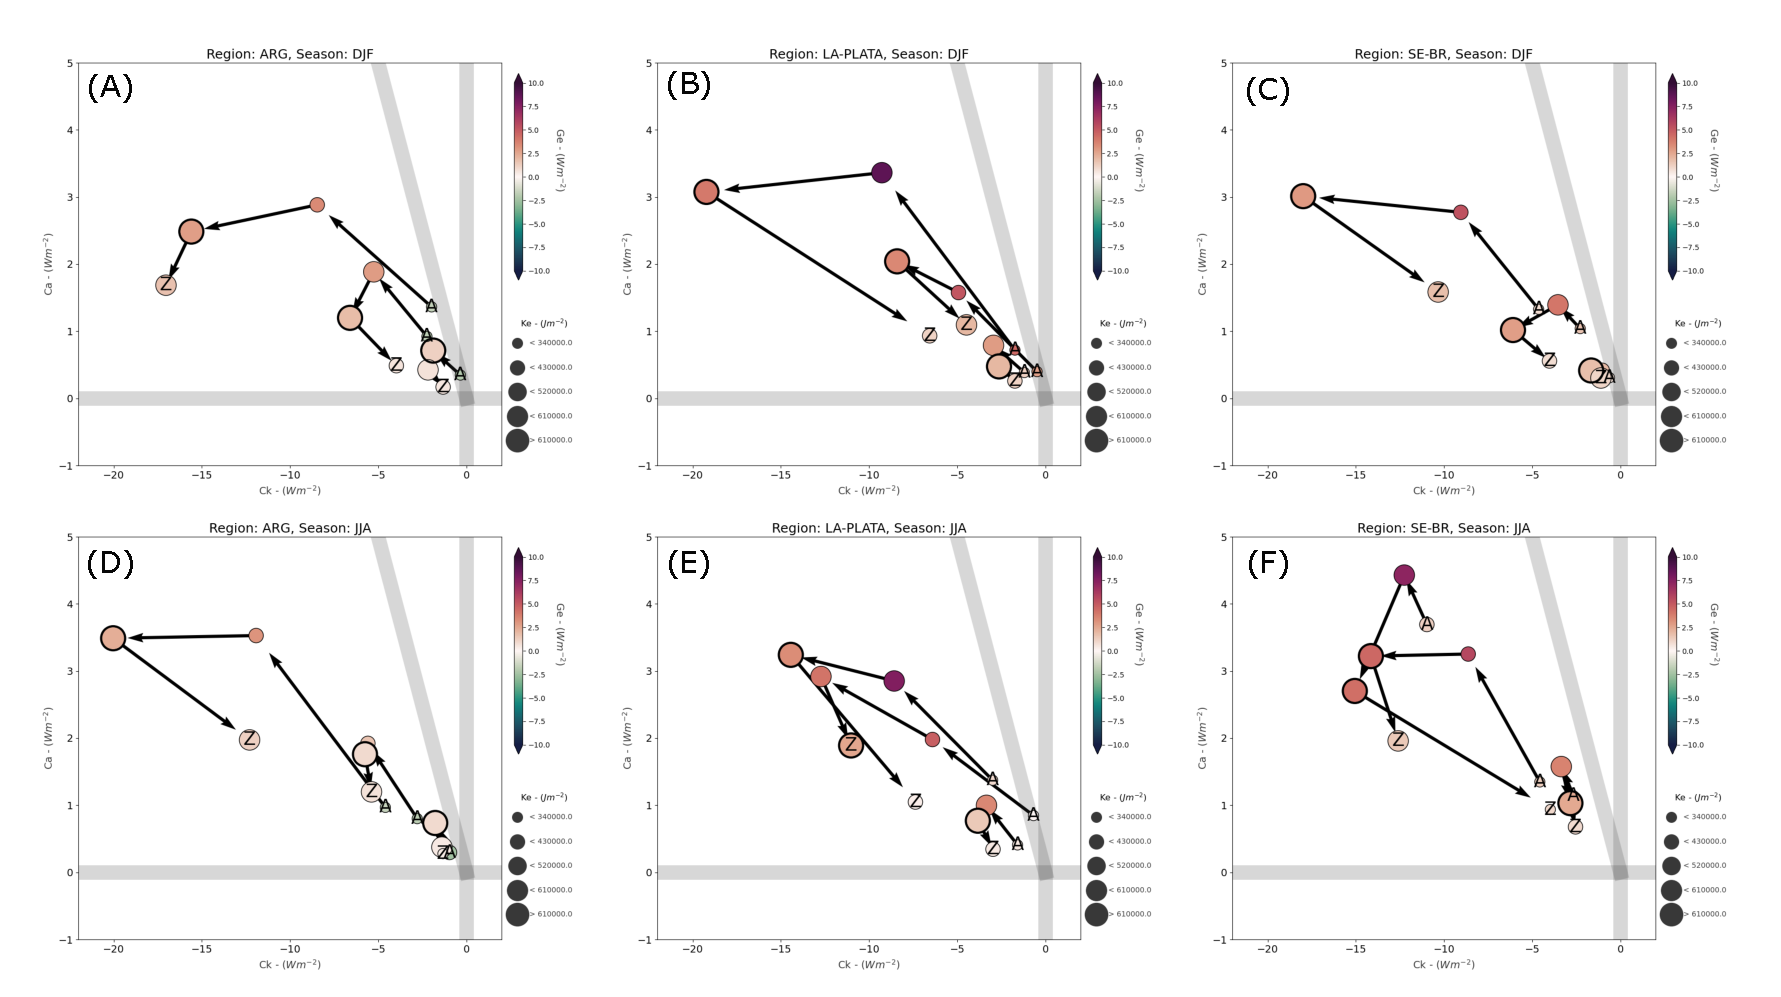
\includegraphics[width=\textwidth]{figs_6/lps_mixed_clusters_IcItDM_seasons_regions.pdf}
\caption[LPS 1 - Clusters - Seasonality and Spatial Variability]{Lorenz Phase Space (LPS) diagram 1 for for the EPs related to the "incipient, intensification, mature, decay" life cycle configuration, across DJF (a, b, c) and JJA months (c, d, e) and for each genesis region in Southwestern Atlantic Region: ARG (a, d), LA-PLATA (b, e) and SE-BR (c, f).}
\label{fig:lps_mixed_clusters_IcItDM_seasons_regions}
\end{figure}

Despite the apparent similarity across the distinct groups, some seasonality and inter-regional variability can be noted. The most notable distinction is in the $G_E$ term: LA-PLATA EPs tend to present lower $G_E$ values compared to the other regions, with ARG presenting relatively high values for both seasons. For both cases, there is no distinction between each season. Meanwhile, for SE-BR, JJA systems present overall higher $G_E$ than DJF systems. For the conversion terms, each group consistently presents EPs that can be interpreted as having lower, medium, and higher energy states, which are very similar among the groups. However, for LA-PLATA and SE-BR during JJA, there are two groups with higher energy states instead.

\begin{figure}[!htbp]
\centering
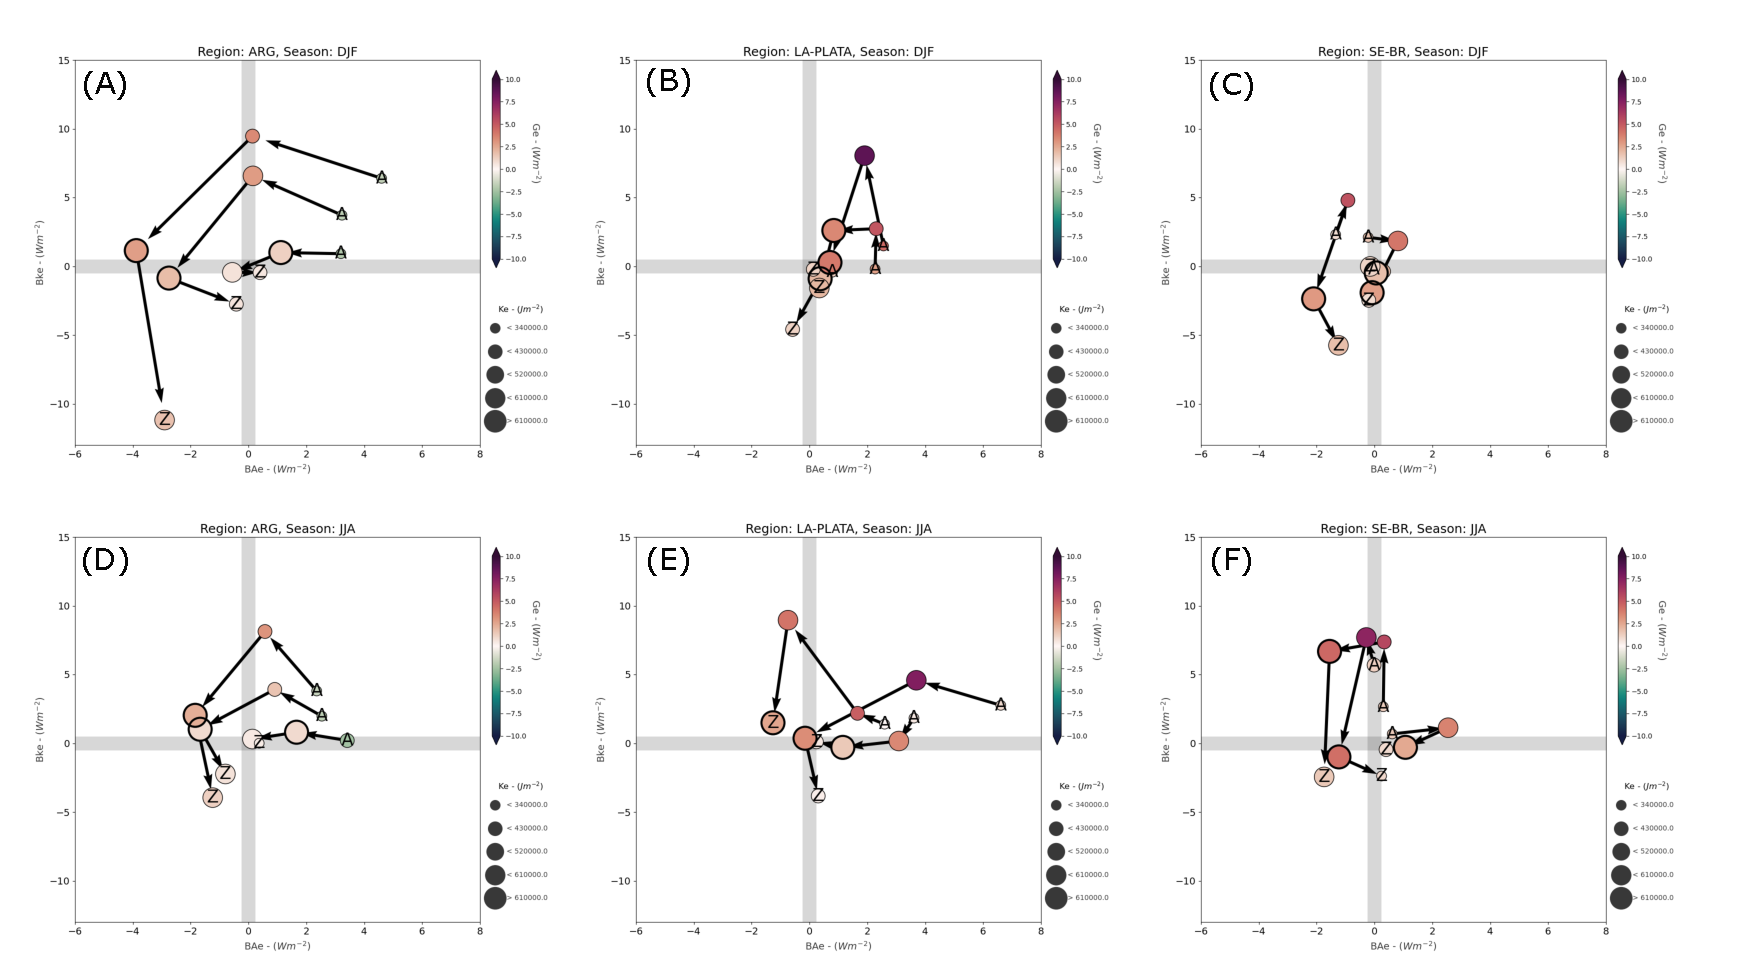
\includegraphics[width=\textwidth]{figs_6/lps_imports_clusters_IcItDM_seasons_regions.pdf}
\caption[LPS 2 - Clusters - Seasonality and Spatial Variability]{Lorenz Phase Space (LPS) diagram 2 for for the EPs related to the "incipient, intensification, mature, decay" life cycle configuration, across DJF (a, b, c) and JJA months (c, d, e) and for each genesis region in Southwestern Atlantic Region: ARG (a, d), LA-PLATA (b, e) and SE-BR (c, f).}
\label{fig:lps_imports_clusters_IcItDM_seasons_regions}
\end{figure}

Meanwhile, for the LPS 2 diagram, the seasonal and inter-regional variability is more evident. For ARG, during both seasons, all EPs initiate with similar imports of $A_E$, with the magnitude of $K_E$ imports increasing in the distinct EPs. During the intensification phase, $K_E$ imports increase, while $A_E$ imports tend to neutrality. In the mature phase, $K_E$ tends to neutrality, while the systems start to export $A_E$. Lastly, in the decay stage, the boundary terms tend to neutrality, except for one cluster, where there are relatively high exports of $K_E$, accompanied by lesser exports of $A_E$.

For LA-PLATA during DJF, two clusters initiate importing $A_E$, with $K_E$ imports increasing during the intensification phase. These imports are higher for one of the EPs. For the remaining phases and the other EP, the boundary terms tend to neutrality. For JJA, one cluster begins with $A_E$ imports, tending to neutrality in later phases. Meanwhile, another cluster starts with high imports of $A_E$, with $K_E$ imports increasing but still moderate in the intensification phase, and both terms tending to neutrality later. For the remaining EP, there are initial imports of $A_E$, high $K_E$ imports in the mature phase, and then finishing near neutrality.

Lastly, for SE-BR, the imports, especially of $A_E$, seem to be of lesser importance. For DJF, all but one EP present neutrality for the import of both forms of energy, with the exception related to imports of $K_E$ in the initial phases and exports in the mature and decay phases. For JJA, one of the EPs presents neutrality for the boundary terms, except during the intensification phase, which shows modest contributions of $A_E$ imports. The remaining EPs start with neutral $A_E$ imports, with increasing $K_E$ imports during the intensification phase. While for one of the EPs, both terms tend to neutrality after the intensification, for the other, $BA_E$ becomes negative during the mature phase, though it remains small, and $BK_E$ becomes negative during decay.

In conclusion, utilizing K-means clustering, the analysis for different regions — ARG, LA-PLATA, and SE-BR — during austral summer (DJF) and winter (JJA) demonstrates that while overall cyclonic systems generally follow a progression from lower to higher energy states through genesis and intensification, there are regional and seasonal variations. The $G_E$ term showed distinct regional characteristics, with LA-PLATA exhibiting higher values and ARG showing lower values irrespective of the season, whereas SE-BR systems displayed higher $G_E$ during winter. For LA-PLATA, the high $G_E$ values for both seasons align with enhanced moisture transport from the South American Low-Level Jet to this region \citep{marengo2004climatology,drumond2008lagrangian}, which is an important heat and moisture source for cyclones forming in this region \citep{gramcianinov2019properties}. Meanwhile, during winter, the sea-air temperature gradient, due to the colder atmosphere over the warm Brazil Current, enhances sensible heat transfer, which reduces atmospheric static stability and supports convective activity.

Additionally, each region-season group had EPs representing low, medium, and high energy states, with specific variations observed in LA-PLATA and SE-BR during winter. The LPS 2 diagram further highlighted regional differences in energy import/export behaviors, with ARG displaying varied import/export dynamics across life cycle phases, LA-PLATA showing differing patterns between DJF and JJA, and SE-BR generally presenting neutral energy imports/exports with some phase-specific deviations. These findings emphasize the importance of baroclinic and especially barotropic conversions for cyclone development on the SESA region, while imports of both eddy energy forms presents a more pronounced seasonal and inter-regional variability.

\subsection{Energy Patterns - Characteristics}\label{ch:ep_mean_features}

In this section, the main characteristics of the EPs for the "incipient, intensification, mature, decay" life cycle configuration will be analyzed (Figure \ref{fig:lps_energy_patterns_IcItDM}). As in Section \ref{sec:energy_patterns}, these EPs were devised by initializing the K-means algorithm for the LEC results for systems in the dataset. EP1 presented the highest occurrence probability, relating to 52\% of all systems, while EP2 and EP3 present progressively lesser probabilities of 36\% and 11\%, respectively. Even when the K-means algorithm was initialized for only the systems where the minimum relative vorticity is lower than the 0.9 quantile, the detected EPs were very similar to EP1. This indicates a consistency in the energy cycle for the systems within the dataset (Appendix \ref{ap:08}).


\begin{figure}[!htbp]
\centering
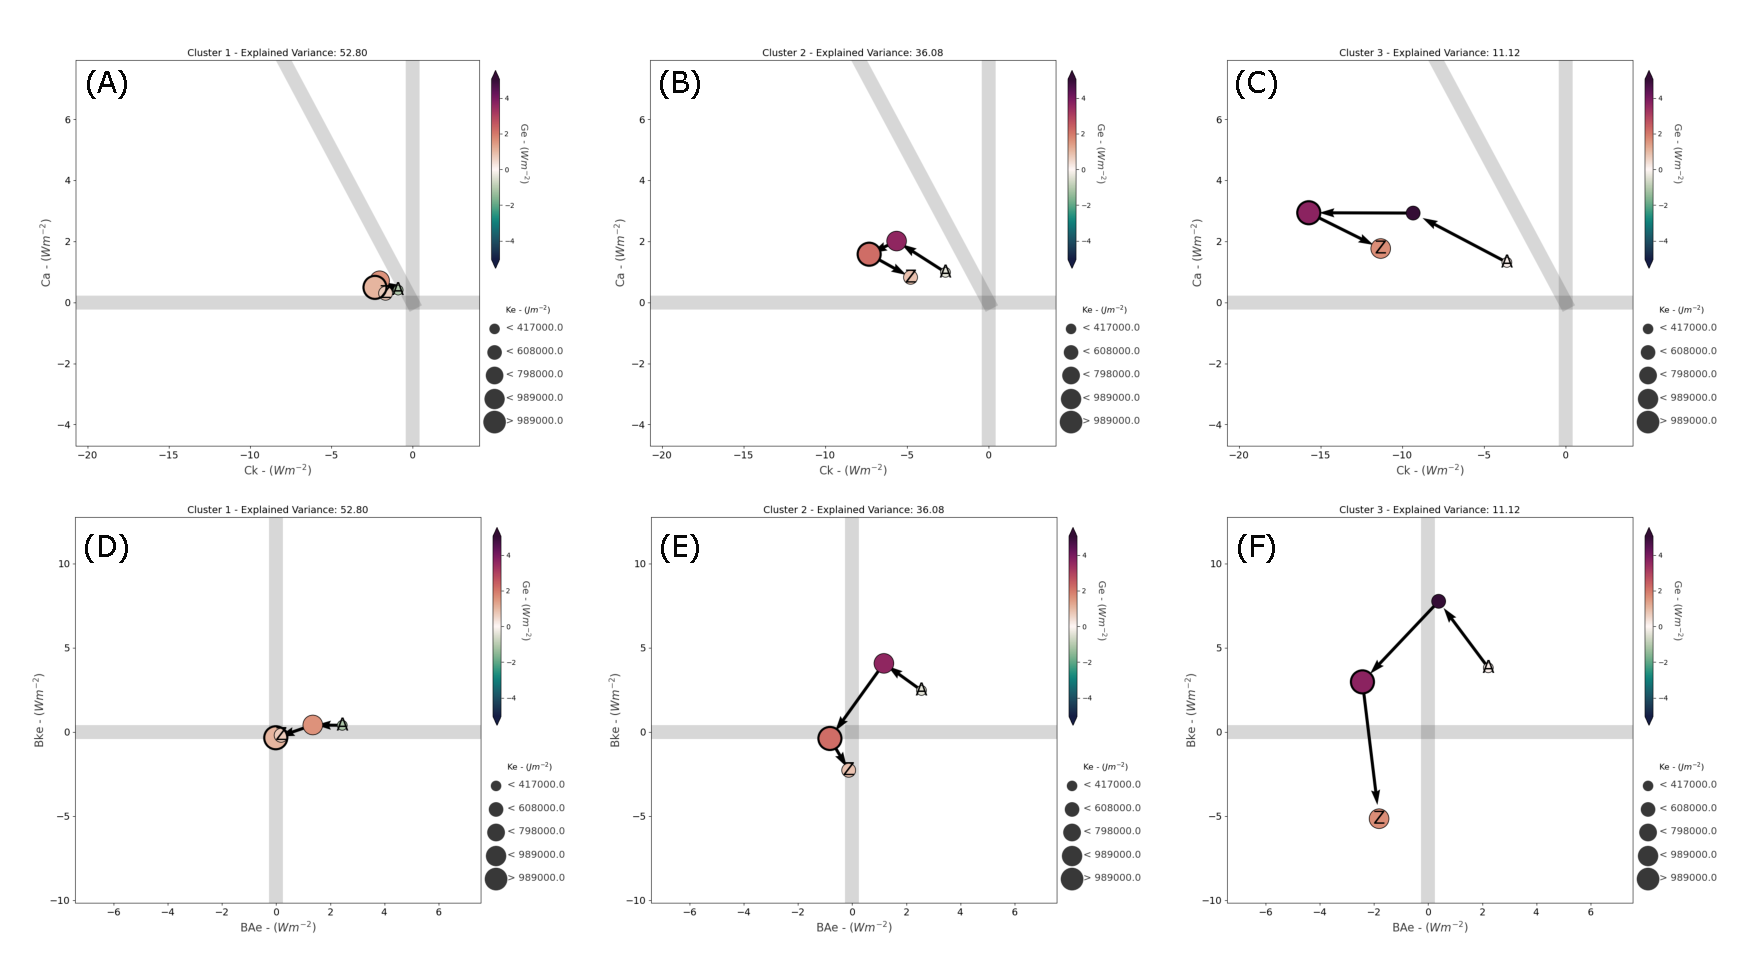
\includegraphics[width=\textwidth]{figs_6/lps_energy_patterns_IcItDM.pdf}
\caption[Energy Patterns]{Lorenz Phase Space (LPS) diagrams 1 (a, b, c) and 2 (d, e, f) for EPs 1 (a, d), 2 (b, e), and 3 (c, f), related to the "incipient, intensification, mature, decay" life cycle configuration.}
\label{fig:lps_energy_patterns_IcItDM}
\end{figure}

As indicated in Sections \ref{sec:energy_patterns} and \ref{sec:energy_patterns_season_region}, the differences found in the EPs are related to their energy states. For the three EPs detected, EP1 has a low energy state, with EPs 2 and 3 presenting progressively higher energy states. Figure \ref{fig:boxplot_vorticity_by_cluster} compares the vorticity distributions across each EP to confirm whether the higher/lower energy states correlate with higher/lower system intensity. The Kruskal-Wallis test was used to assess overall differences in vorticity among the clusters, revealing significant disparities. Subsequently, pairwise comparisons using the Mann-Whitney U test identified specific clusters with significantly different vorticity values. The plot illustrates that the EPs exhibit significantly different vorticity values, as indicated by the stars, which represent p-values from the pairwise comparisons. Therefore, the hypothesis that each EP represents a distinct intensity cyclone category is confirmed.

\begin{figure}[!htbp]
    \centering
    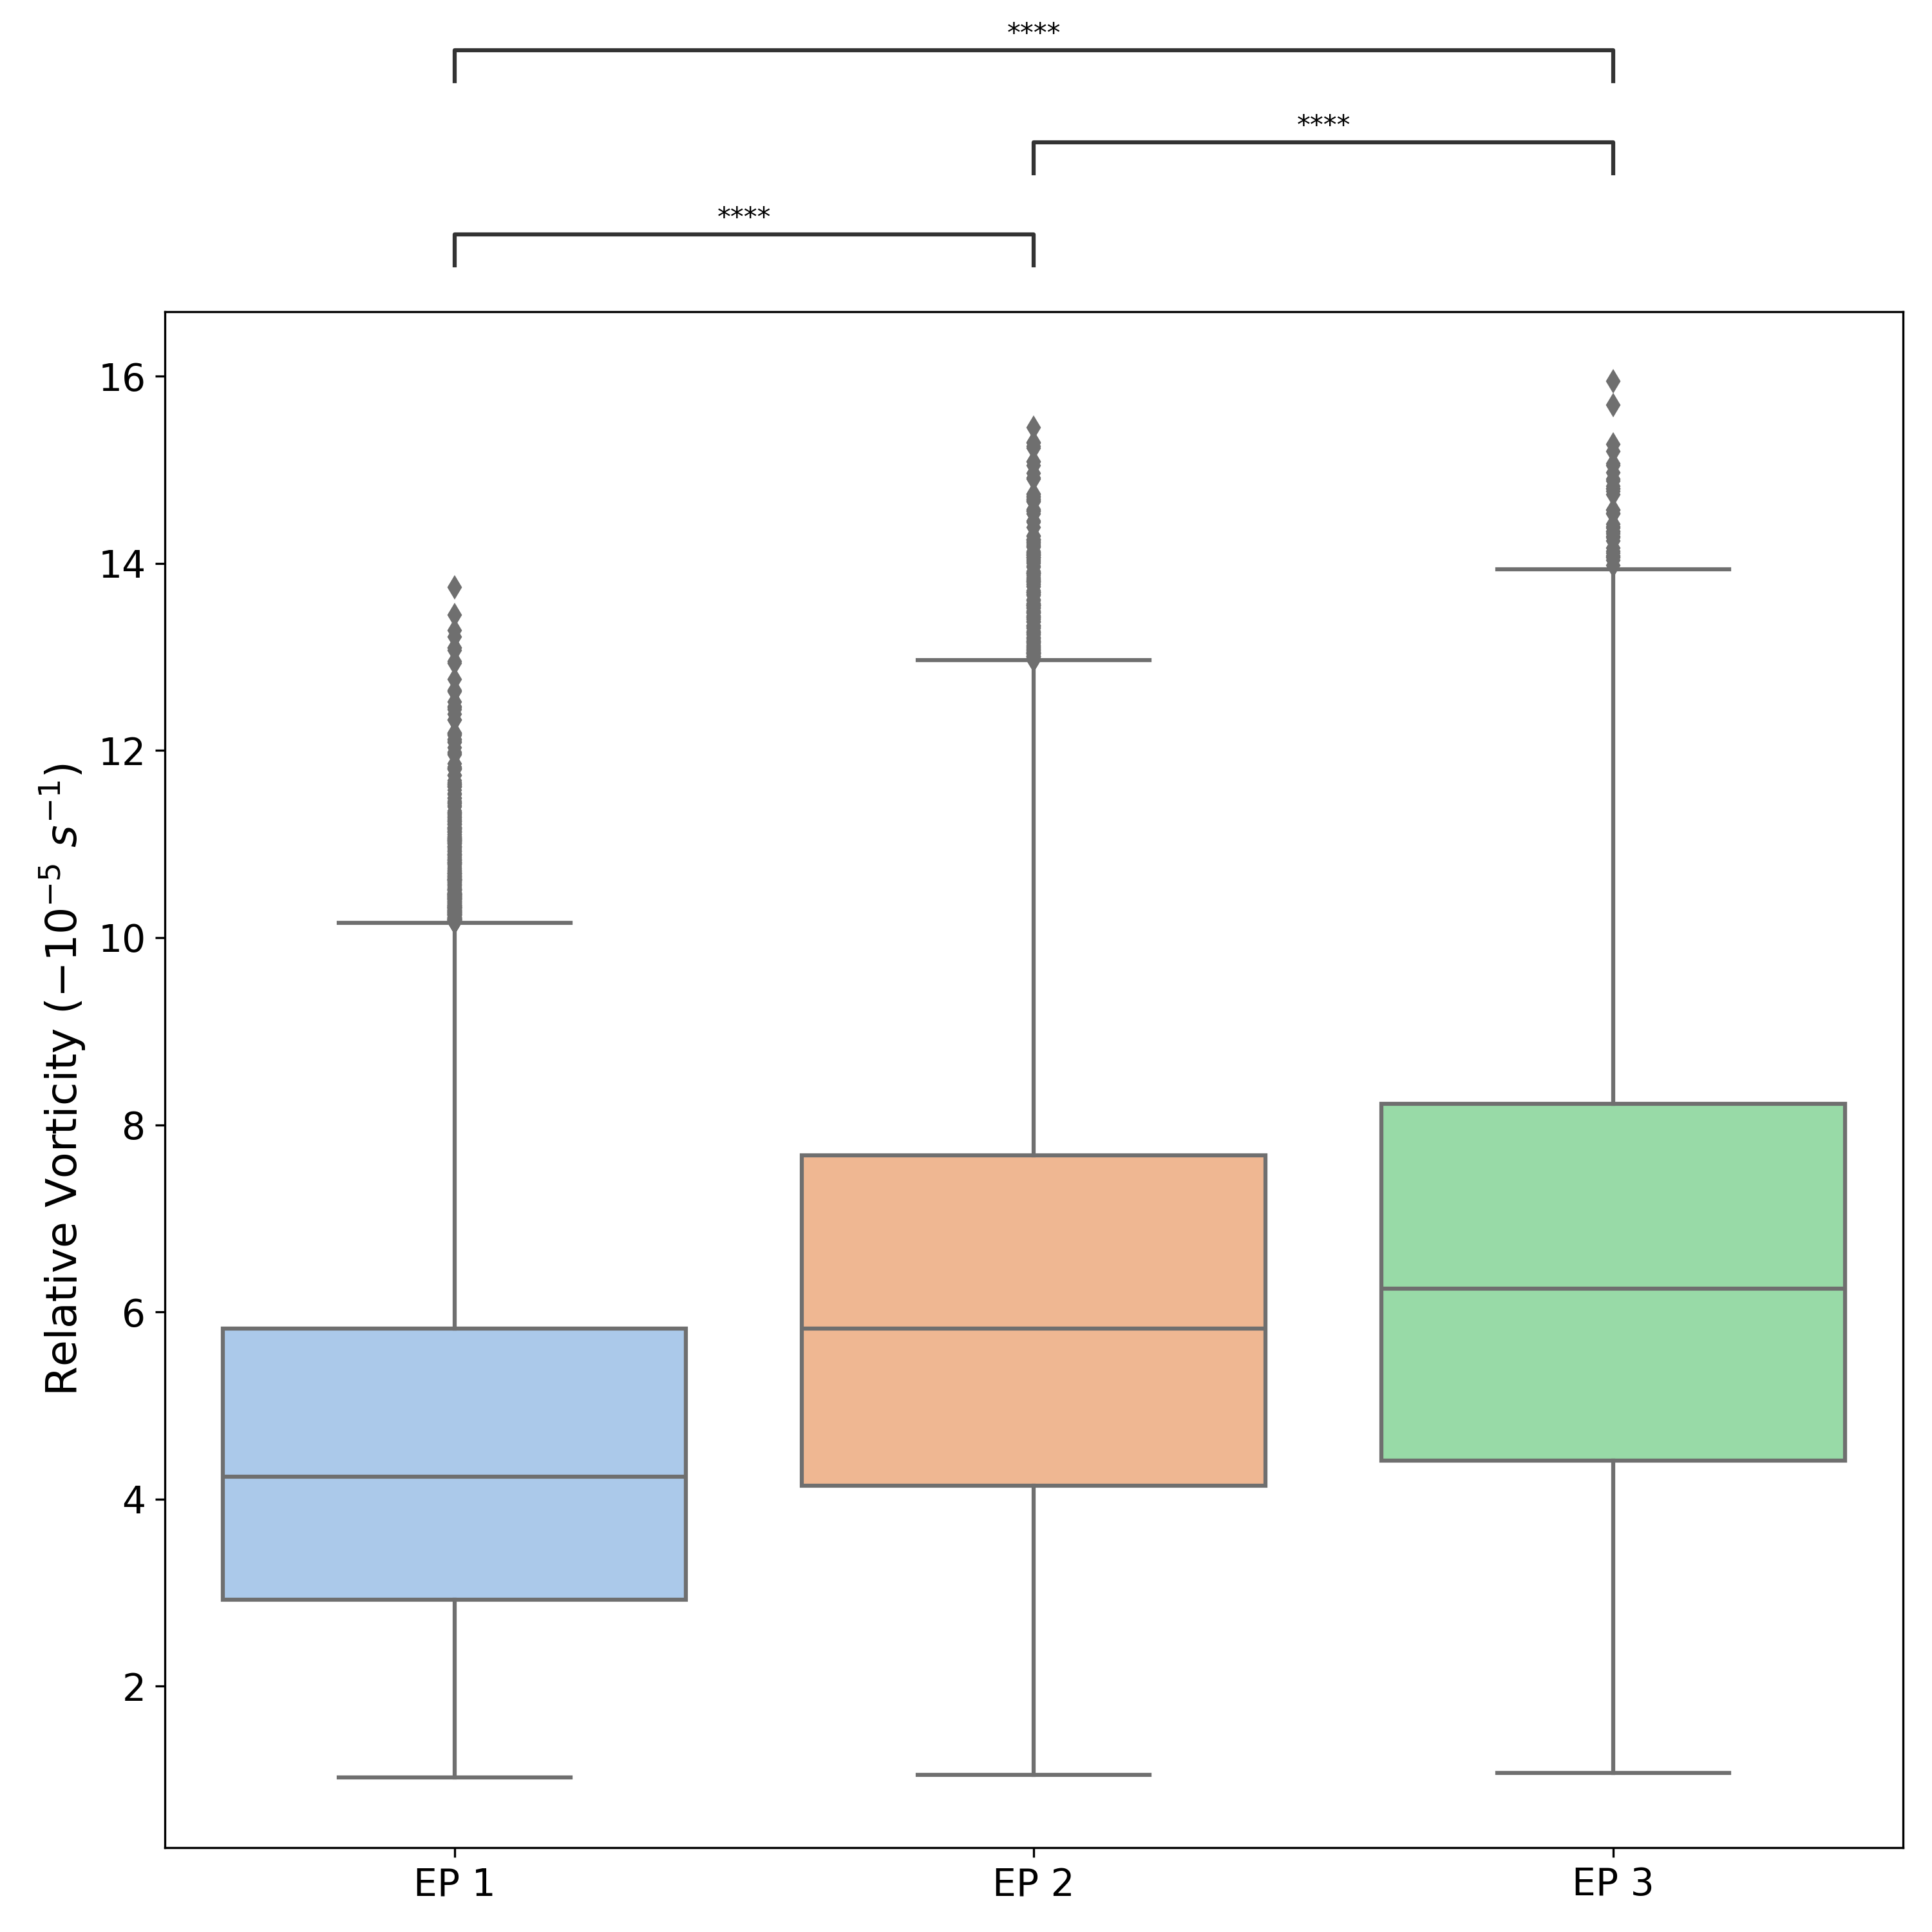
\includegraphics[width=0.6\textwidth]{figs_6/boxplot_vorticity_by_cluster.png}
    \caption[Energy Patterns - Mean Intensity]{Box plot comparing the vorticity distributions among different energy patterns (EPs). The Kruskal-Wallis test was used to determine if there were statistically significant differences in the vorticity distributions across the clusters. Significant differences identified by pairwise Mann-Whitney U tests are annotated on the plot.}
    \label{fig:boxplot_vorticity_by_cluster}
\end{figure}

In Figure \ref{fig:ep_frequencies_by_region}, the relative frequency of each EP for each genesis region is represented. For ARG and SE-BR, the regional behavior is similar to the overall frequencies, with the most intense systems (EP3) presenting lower frequencies and relative frequencies increasing progressively for EP2 and EP1. However, for LA-PLATA, EP2 presents a higher relative frequency than EP1. Additionally, this region shows the highest relative frequencies for EP2 and EP3, indicating that it often generates more intense systems than the others. 

\begin{figure}[!htbp]
    \centering
    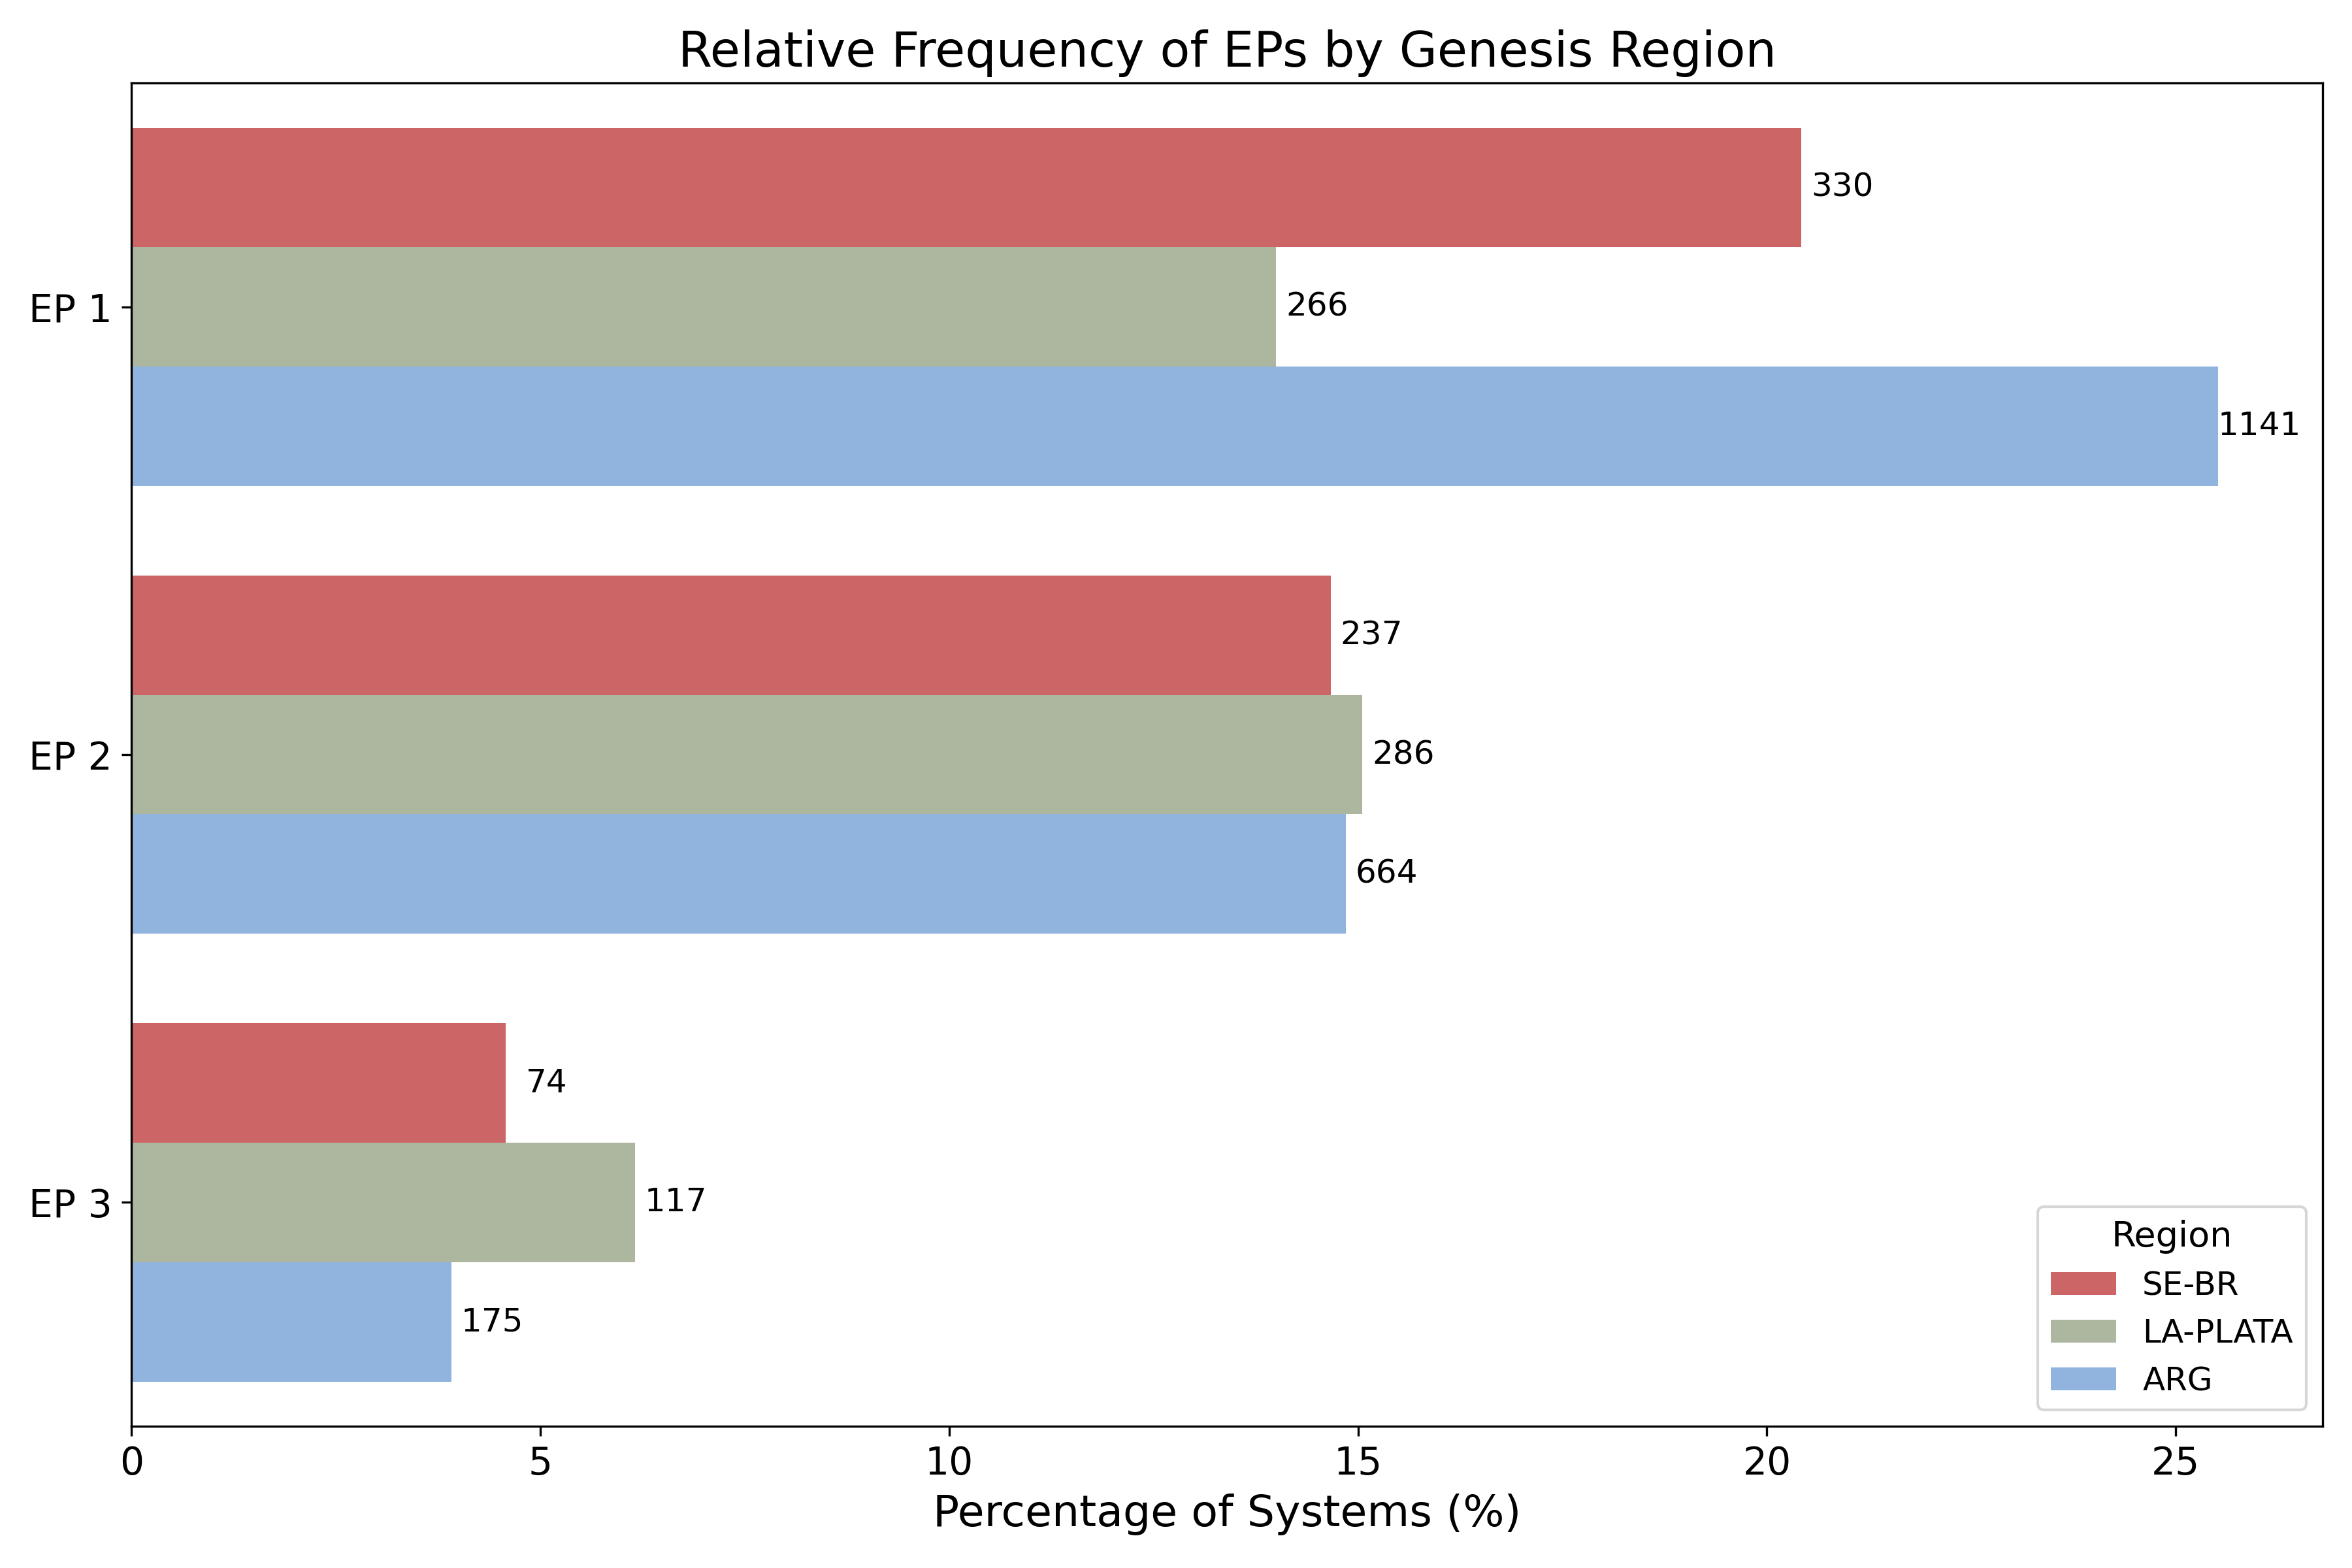
\includegraphics[width=0.6\textwidth]{figs_6/ep_frequencies_by_region.png}
    \caption[Energy Patterns - Frequency by Region]{Relative regional variability of each energy pattern (EP) for each genesis region in the Southwestern Atlantic. The annotations alongside each bar represent the total count for each EP for the given region.}
    \label{fig:ep_frequencies_by_region}
\end{figure}

Figure \ref{fig:lps_seasonality} displays the seasonality of each EP, represented as the counts of the cyclogenesis events associated with each EP. These events were defined as the first time step of the track for each system in the dataset. The results presented here differ from those presented in Section \ref{sec:energy_patterns_season_region}, as there the EPs for each region-season group were determined independently, while here, the seasonal behavior of the mean EPs is observed. 

Overall, there is a higher occurrence of EP1 in DJF, followed by SON. EP2 presents a more homogeneous distribution across seasons, while EP3 is especially active during JJA, with low activity in DJF. This indicates a higher occurrence of stronger cyclonic systems, with more active energy conversion and convective activity during JJA, and weaker systems during DJF. This result is corroborated by Chapter \ref{ch:life_cycle} (Figure \ref{fig:pdf_mean_vorticity}), which indicates the occurrence of stronger systems during JJA than DJF.


\begin{figure}[!htbp]
    \centering
    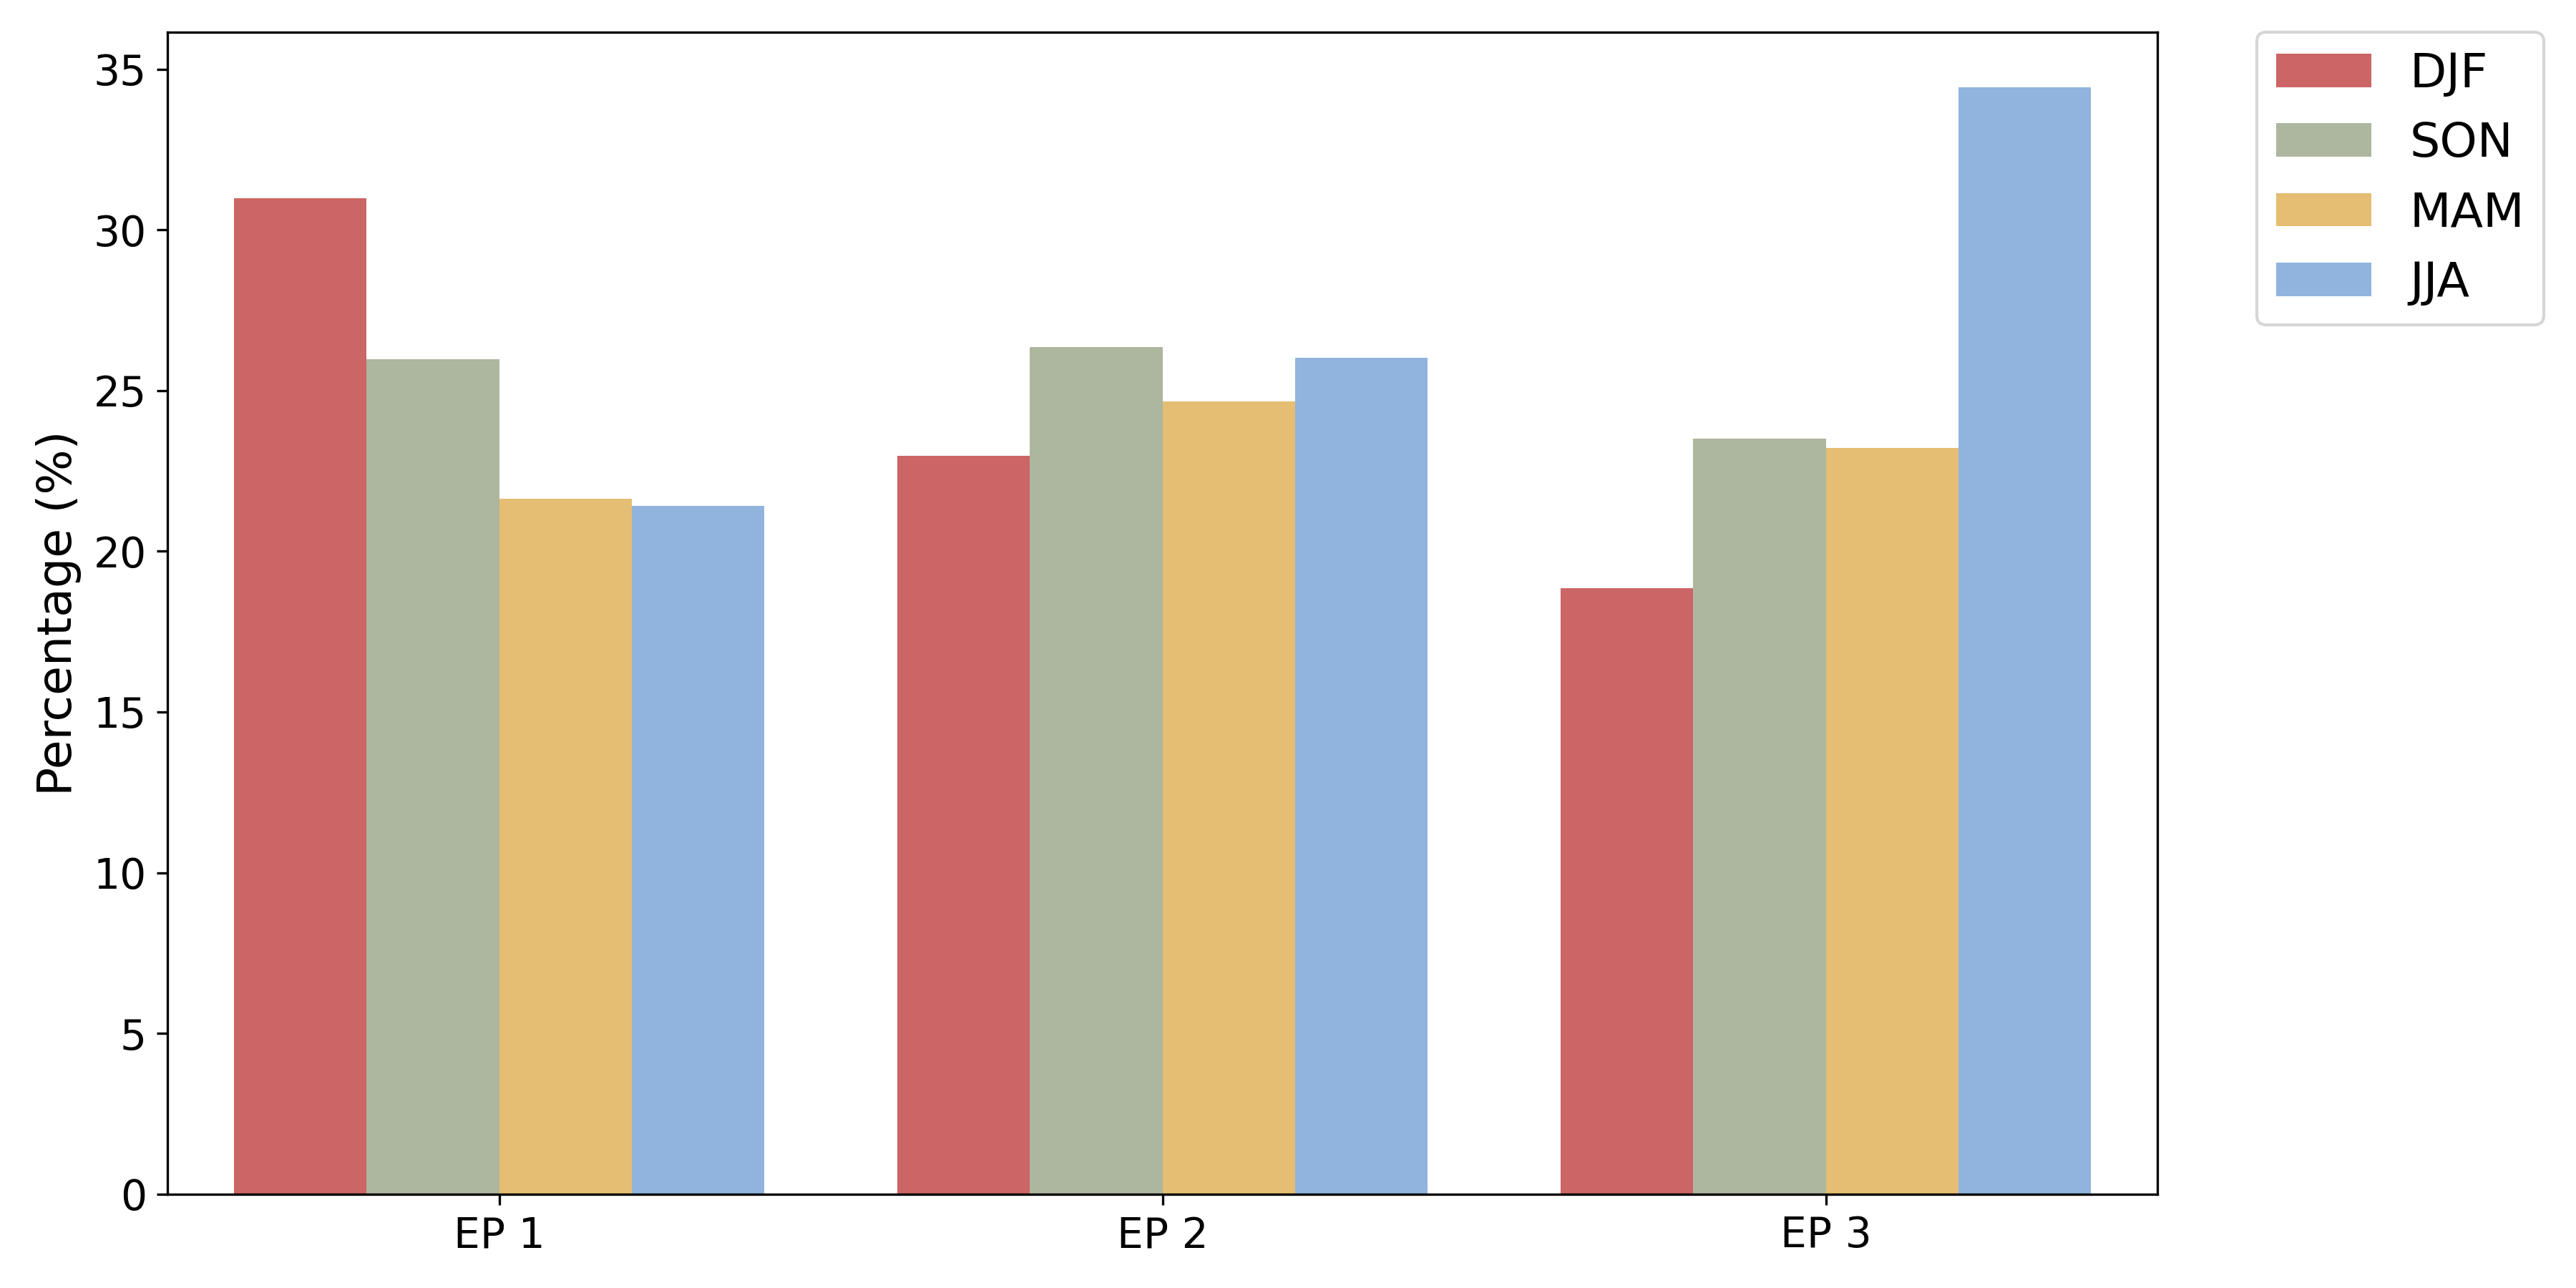
\includegraphics[width=0.6\textwidth]{figs_6/lps_seasonality.png}
    \caption[Energy Patterns - Seasonality]{Box plot comparing the Seasonality of energy petterns (EPs) in the Southwestern Atlantic region, with the y-axis representing the percentage of cyclones occurring in each season within the respective EP.}
    \label{fig:lps_seasonality}
\end{figure}

Figure \ref{fig:lps_interannual_variability} illustrates the interannual variability of each EP from 1979 to 2020. While the results do not indicate clear trends in EP occurrence over the years, they do reflect significant interannual differences. Notably, EP3 exhibits higher variability, with relative yearly frequencies ranging from 1\% to 5\%, whereas EPs 1 and 2 demonstrate more homogeneous behavior, typically with relative frequencies between 2\% and 3\%. Exceptionally high frequencies of EP1 were observed in 1996 and 2013, with particularly low frequencies in 2016. The relative importance of EP1 is noteworthy due to the impacts caused by strong cyclonic systems in coastal regions \citep{de2021ocean,cardoso2022synoptic,leal2023identification}. This variability could suggest low-frequency climate influences on cyclone genesis and development in the South Atlantic region, such as those from the El Niño-Southern Oscillation and the Southern Annular Mode, which will be explored in future studies.


\begin{figure}[!htbp]
    \centering
    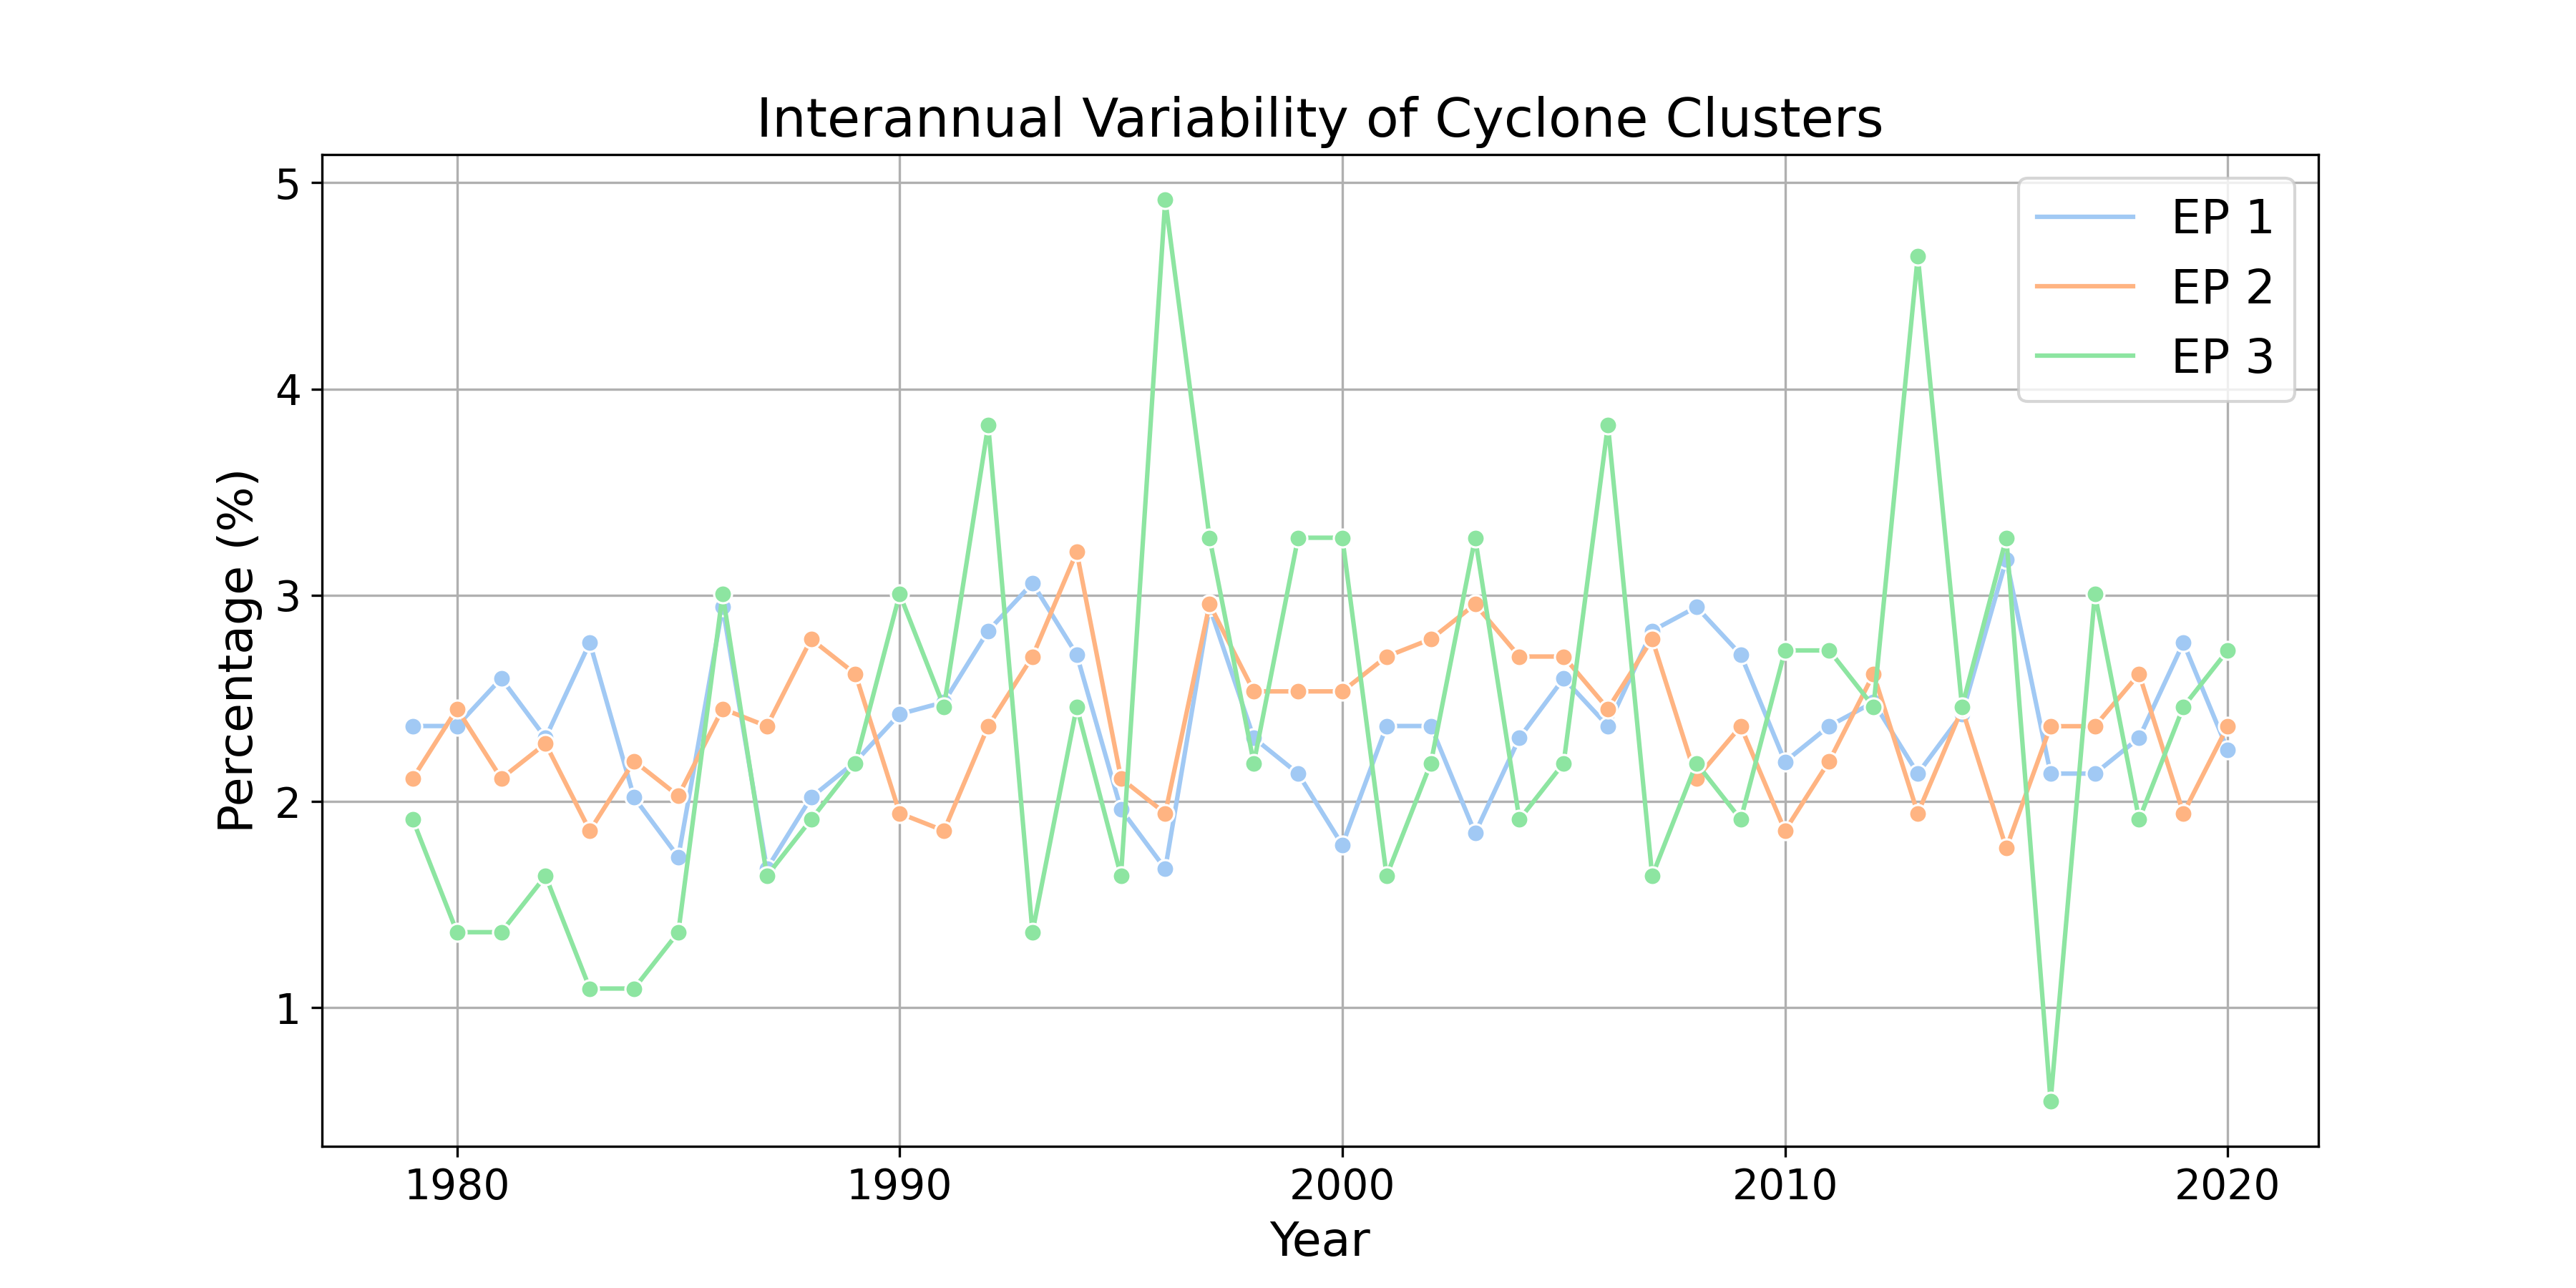
\includegraphics[width=\textwidth]{figs_6/lps_interannual_variability.png}
    \caption[Energy Patterns - Interannual Variability]{Interannual variability of energy patterns (EPs) from 1979 to 2020. The y-axis represents the percentage of cyclones each year for different EPs, normalized to total cyclones numbers for each EP.}
    \label{fig:lps_interannual_variability}
\end{figure}

\section{Physical Mechanisms}

\subsection{Barotropic and Baroclinic Instability}\label{sec:ibt_ibc}

Through Chapter \ref{ch:energetics} and Section \ref{sec:lps} the results for the LEC for all systems forming on the cyclogenesis regions located near South America, for the period ranging from 1979 and 2020 were explored and discussed. The results indicates an ominous importance of baroclinic and barotropic conversions for the development of the cyclonic systems analysed. The role of baroclinic instability on mid-latitude cyclogenesis, and the further development of these systems, is deeply established on the literature \citep{bjerknes1922life,eady1949long,charney1947dynamics,petterssen1971development,hoskins1990existence}. However, the relationship of barotropic instability and extratropical cyclogenesis and development is not often explored. 

Given that the relationship between extratropical cyclones and barotropic instability might challenge the common notions in the scientific literature, the current section aims to demonstrate the validity of the presented results. An analysis of the Rayleigh-Kuo criterion will be performed to determine if barotropic instability is indeed occurring in the systems analyzed (Section \ref{sec:ibc_ibt_analysis}). For this, only the systems associated with EP1 will be used, as they present the highest energy states (Figure \ref{fig:lps_energy_patterns_IcItDM}). These systems tracks are represented on Appendix \ref{ap:09}. Also, only data for the intensification phase will be used, as these conversions are often strong during this phase and for ensuring the dynamics related to the system intensification is captured.

Firstly, the vertical levels where the baroclinic and barotropic conversions are most intense are assessed. Figure \ref{fig:levels_ibc_ibt} displays the vertical distribution of $C_A$ and $C_E$ terms for EP1 systems. It can be seen that for $C_A$, the most positive values (indicating baroclinic conversions) are found near the surface, at 1000 hPa. This agrees with the Polar Front Theory, which suggests that low-level baroclinicity initiates cyclogenesis and maintains cyclone development \citep{bjerknes1922life}, as well as with Petterssen type A cyclones \citep{petterssen1971development}. Positive mean values can also be seen for $C_A$ on the upper troposphere, but with smaller overall magnitudes. For barotropic conversions, however, the lowest values ($K_Z \rightarrow K_E$ conversions) are found in the upper troposphere, with the lowest mean values at 300 hPa. This vertical distribution of $C_K$ is consistent with the mean jet vertical positioning, indicating the importance of upper-level jet streams in providing kinetic energy to the eddy motions. 

\begin{figure}[!htbp]
    \centering
    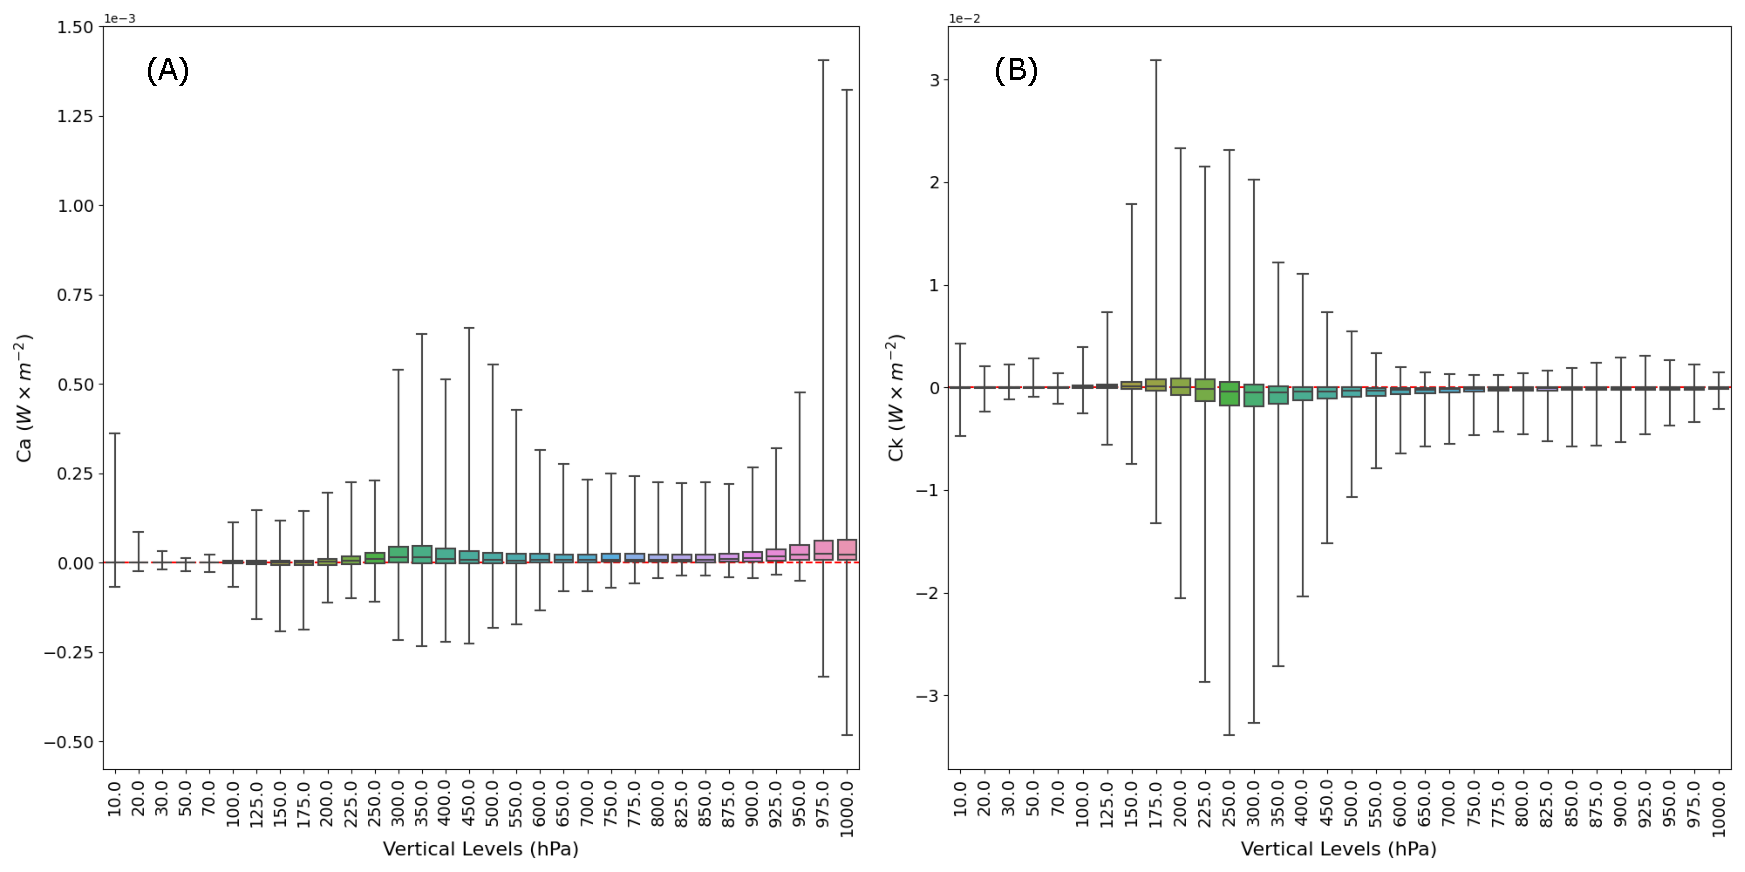
\includegraphics[width=\textwidth]{figs_6/levels_ibc_ibt.pdf}
    \caption[Ca and Ck - Vertical Distribution]{Boxplots for each vertical level, for (A) $C_A$ and (B) $C_E$ terms, for energy pattern (EP) 1 systems.}
    \label{fig:levels_ibc_ibt}
\end{figure}

Given such vertical distributions for $C_A$ and $C_K$ terms, composites of meteorological fields were prepared to assess the occurrence of baroclinic and classical barotropic instabilities at these distinct levels. For this purpose, the maximum Eady Growth Rate (EGR) fields were evaluated and the Rayleigh-Kuo (RK) criterion was applied. These metrics are shown in Figure \ref{fig:ibc_ibt_panel}, for the composites of all systems related to EP1, across the mean fields during the intensification phase.

Figure \ref{fig:ibc_ibt_panel}a demonstrates the RK criterion, showing the derivative of absolute vorticity ($\eta$) at 250 hPa with respect to latitude. A strong meridional gradient of $\eta$ is evident, with a sign reversal near the cyclone center, satisfying the RK criterion and indicating that barotropic instability might indeed be occurring. Figure \ref{fig:ibc_ibt_panel}b shows the zonally averaged meridional derivative of $\eta$, providing a clearer illustration of the RK criterion.

Meanwhile, Figure \ref{fig:ibc_ibt_panel}c shows the potential vorticity composites. Here, the 900 hPa level was used instead of 1000 hPa due to artifacts related to the vertical coordinate interpolation from height to isobaric levels when computing the EGR fields. This figure reveals an area of intense cyclonic activity in the middle of the Semi-Lagrangian domain, associated with low-pressure systems and significant vorticity. Figure \ref{fig:ibc_ibt_panel}d shows the EGR composites, demonstrating a strong baroclinic region east/southeast of the cyclone centers, indicating regions susceptible to baroclinic instability, which is on agreement with mean cyclone displacement on SESA region \citep{hoskins2005new,gramcianinov2019properties}. These areas coincide with sharp PV gradients observed in Figure \ref{fig:ibc_ibt_panel}c, reinforcing these areas as susceptible to cyclonic development.

\begin{figure}[!htbp]
    \centering
    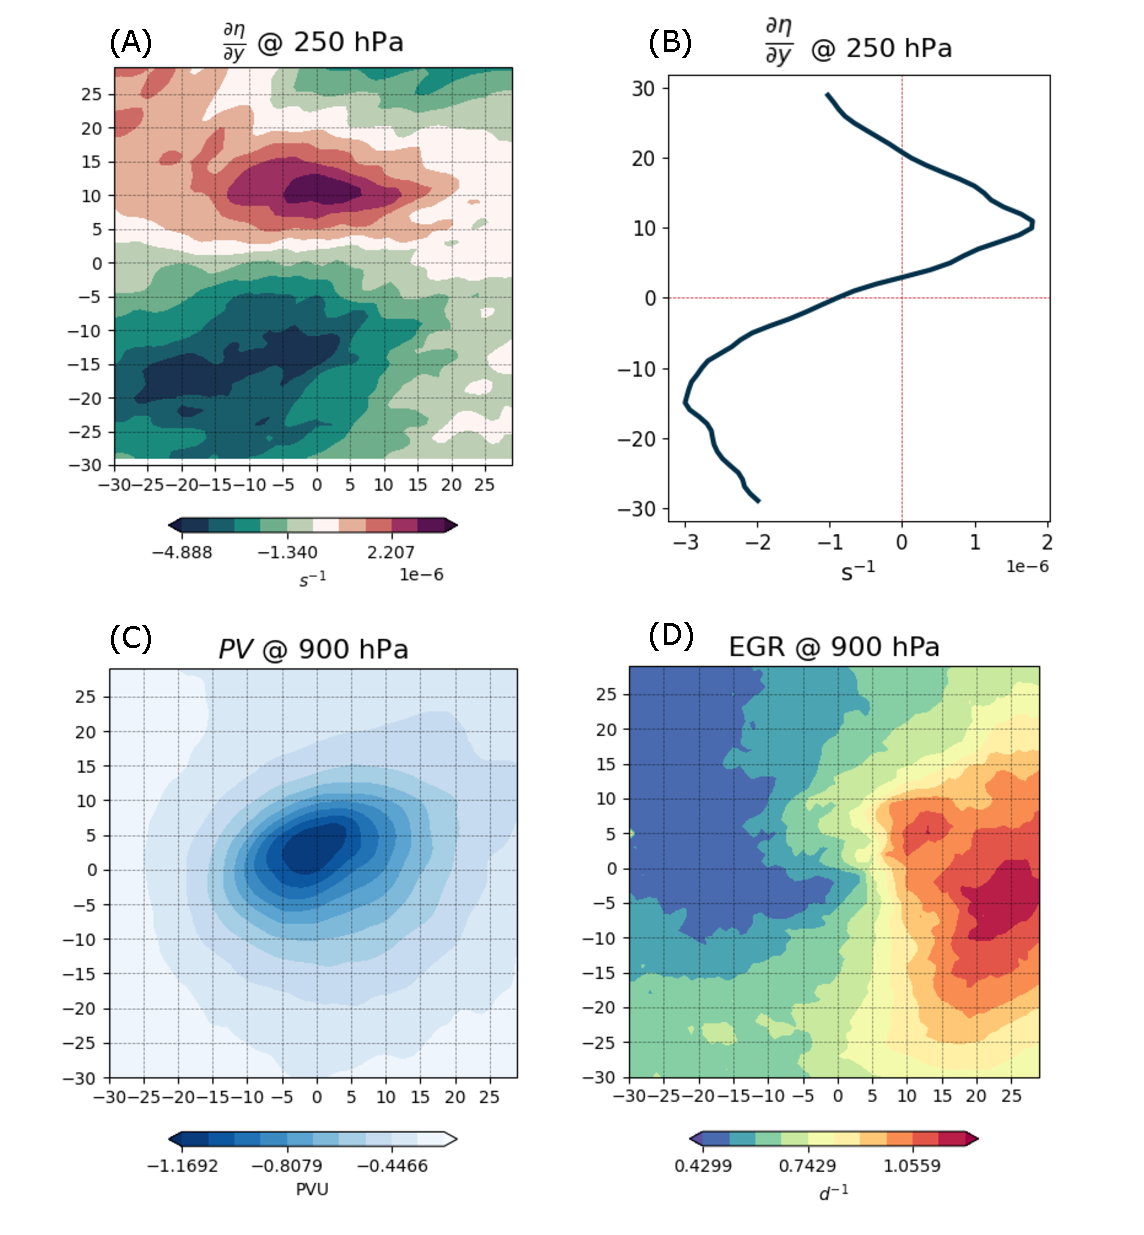
\includegraphics[width=\textwidth]{figs_6/ibc_ibt_panel.pdf}
    \caption[Rayleigh Criterion and EGR]{Composite Analysis of Barotropic and Baroclinic Instabilities. (a) The derivative of absolute vorticity ($\eta$) at 250 hPa with respect to latitude, illustrating the Rayleigh-Kuo (RK) criterion. (b) Zonally averaged meridional derivative of $\eta$. (c) Potential vorticity (PV) composites at 900 hPa. (d) Maximum Eady Growth Rate (EGR) composites at 900 hPa.}
    \label{fig:ibc_ibt_panel}
\end{figure}

These results reinforce the conclusions from Chapter \ref{ch:energetics} and Section \ref{sec:lps} that both baroclinic and barotropic instabilities act in consonance for cyclone genesis and development in the SESA region. While barotropic instability acts in the upper troposphere, extracting energy from the jets for cyclonic development, baroclinic instability in the lower troposphere transforms the meridional temperature gradients into eddy potential energy, ultimately feeding eddy kinetic energy.

\citet{hoskins1985use} described the general situation where an upper-level PV cyclone acting over a low-level baroclinic region triggers surface cyclogenesis. The results shown here indicate that the baroclinic chain is initially stronger, with barotropic conversions increasing afterward and peaking at the cyclone's mature phase (Section \ref{sec:eof_phases}). If these baroclinic conversions occur at lower levels, while barotropic conversions occur at upper levels, this suggests a distinct mechanism as proposed by \citet{hoskins1985use}, although this requires further exploration.

It is important to recognize, however, that the approach adopted has its limitations. Firstly, the Rayleigh–Kuo criterion is derived from a linear stability analysis, which assumes small perturbations to the basic flow and does not account for the nonlinear processes that can become significant as instabilities grow and evolve. It is also based on idealized conditions, such as an inviscid (non-viscous) and incompressible flow, whereas real atmospheric and oceanic flows are neither purely inviscid nor incompressible. Furthermore, it is a necessary but insufficient criterion for instability (see \citet{read2020baroclinic}). However, the overall $K_Z \rightarrow K_E$ conversions, in consonance with satisfying the RK criterion, provide strong evidence for barotropic instability being related to cyclone development in the SESA region.

\subsection{Comparing with the Fixed Framework}

The results shown so far indicate that barotropic instability plays an important role in extratropical cyclone development. While some studies have detected this phenomenon, it has not been fully explored in the literature. Why has this important aspect received limited attention? As the use of the Semi-Lagrangian Framework is rarely seen in the literature, the answer might lie in the intrinsic differences between the Semi-Lagrangian and the more commonly used Fixed Framework.


This section aims to explore this dichotomy. Here, the same systems analyzed in Section \ref{sec:ibt_ibc} (the systems related to EP1) are analyzed, but now using the Fixed Framework. In Figure \ref{fig:lps_fixed_means} it is shown the LPS diagram 1 for EP1 systems mean values. In this case, the LEC of EP1 systems were computed using the Fixed Framework and then, for each development phase (incipient, intensification, mature and decay), the mean values were computed, excluding outliers. The LPS indicates a mean behaviour where the cyclones have genesis and intensify with shared contributions from moist baroclinic and barotropic conversions, with the barotropic conversions becoming more important on the mature and decay phases. These results indicate that the Fixed Framework also evidences the importance of barotropic conversions on cyclonic systems in SESA region, but with lower mean magnitude than the Semi-Lagrangian method. Also, caution should be taken into examining the results form the Fixed Framework, as, for EP1 cases there were systems with high horizontal displacement (Appendix \ref{ap:09}), therefore their computational domain encompassed almost entirely the Southern Atlantic region and most certainly more than one cyclonic system was acting on that domain during the analysis.

\begin{figure}[!htbp]
\centering
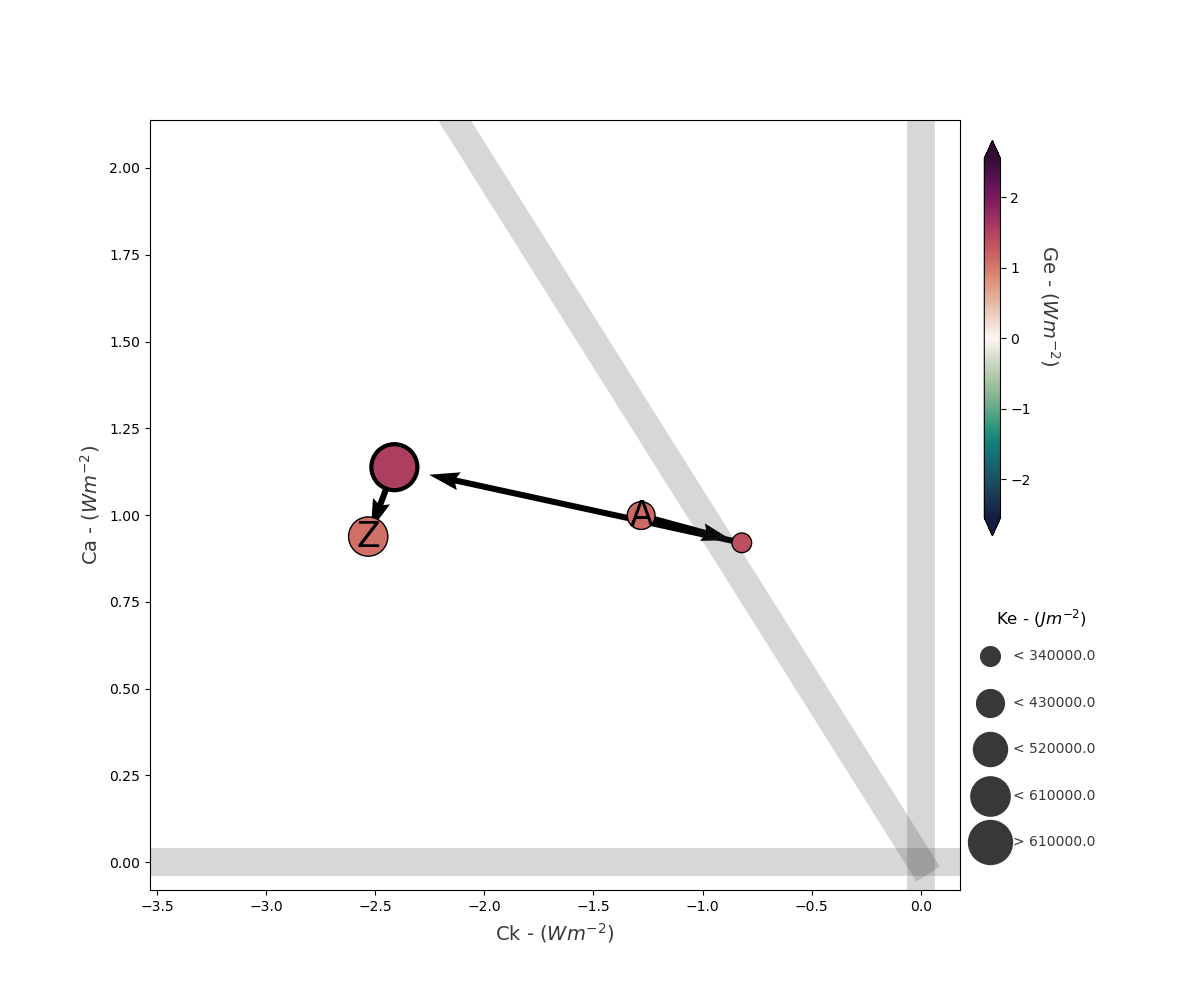
\includegraphics[width=\textwidth]{figs_6/lps_fixed_means.png}
\caption[LPS for Fixed Framework Systems]{Lorenz Phase Space (LPS) diagram 1 for energy pattern (EP) 1 systems mean values for each phase (incipient, intensification, mature and decay), computed using a fixed framework.}
\label{fig:lps_fixed_means}
\end{figure}

The following step was to defined to investigate the role of the LEC methodology in affecting the magnitude of the barotropic and baroclinic conversions. Figure \ref{fig:ibc_ibt_panel_fixed} displays the same analysis as Figure \ref{fig:ibc_ibt_panel}, but for the composites using the Fixed Framework. Although there are sign reversals in the meridional $\eta$ derivative zonally averaged values, the spatial field displays a less cohesive spatial field compared to the Semi-Lagrangian results. For the PV field, an increase in its magnitude can be seen poleward, which is the expected behavior. Additionally, for EGR, a modest baroclinic region can be seen from the central to eastern parts of the domain. This is again the expected behavior for this region, with magnitudes comparable to the climatological values \citep{de2023storm}. There is also a spot of high baroclinicity to the west, near the interpolated domain area equivalent to the ARG cyclogenesis region. Although this high baroclinic region in the west might be related to cyclogenesis in the Southwestern region, the composites do not show a clear signature of cyclonic development as in Figure \ref{fig:ibc_ibt_panel}.

\begin{figure}[!htbp]
    \centering
    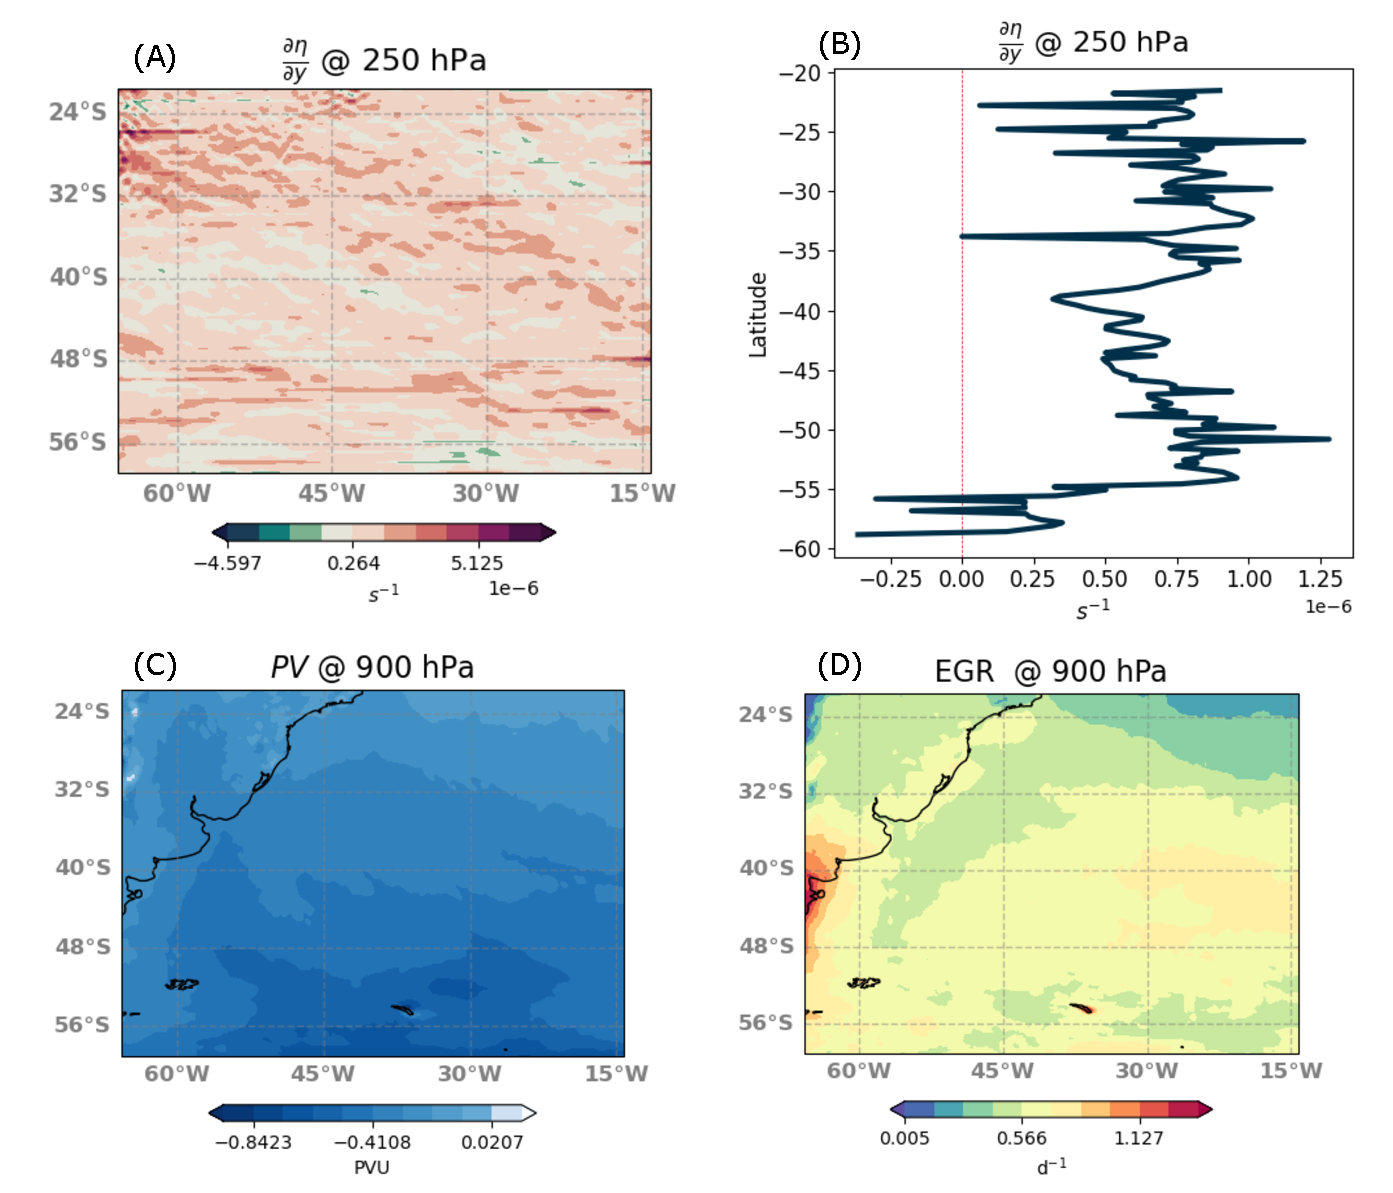
\includegraphics[width=\textwidth]{figs_6/ibc_ibt_panel_fixed.pdf}
    \caption[Rayleigh Criterion and EGR - Fixed Framework]{Composite Analysis of Barotropic and Baroclinic Instabilities using the Fixed Framework. (a) The derivative of absolute vorticity ($\eta$) at 250 hPa with respect to latitude, illustrating the Rayleigh-Kuo (RK) criterion. (b) Zonally averaged meridional derivative of $\eta$. (c) Potential vorticity (PV) composites at 900 hPa. (d) Maximum Eady Growth Rate (EGR) composites at 900 hPa.}
    \label{fig:ibc_ibt_panel_fixed}
\end{figure}

To better illustrate the effect of the methodology on the results, let us examine a case study comparing the results for both methodologies. Figure \ref{fig:panel_compare_fixed_sl} shows the results for a system with genesis on March 1, 1982, during the period when the barotropic conversions were most intense. Figure \ref{fig:panel_compare_fixed_sl}a illustrates the computational domain used for running the Fixed Framework, while its track is displayed in Figure \ref{fig:panel_compare_fixed_sl}b, along with the Semi-Lagrangian domain defined for that given time step.

The EGR fields for the Fixed domain display a maximum in the southern parts of South America, near $70^\circ W$ (Figure \ref{fig:panel_compare_fixed_sl}c), while the cyclonic center is at $36^\circ W$ (Figure \ref{fig:panel_compare_fixed_sl}d). Here, the EGR fields for 875 hPa are displayed due to the occurrence of artifacts related to the vertical interpolation in the 900 hPa fields. Thus, despite the mean EGR values for the Fixed domain being higher (0.55 $day^{-1}$) than those for the Semi-Lagrangian domain (0.45 $day^{-1}$), these values are related to the maximum away from the cyclone center, therefore reinforcing the reasoning that the use of the Fixed Framework captures dynamics unrelated to cyclonic system development. For the meridional derivative of $\eta$, regions inside the Fixed Framework satisfying the RK criterion can be seen, such as in Southern Argentina (Figure \ref{fig:panel_compare_fixed_sl}e). However, inside the Semi-Lagrangian domain, near the cyclone center, this effect is more pronounced (Figure \ref{fig:panel_compare_fixed_sl}f).

\begin{figure}[!htbp]
    \centering
    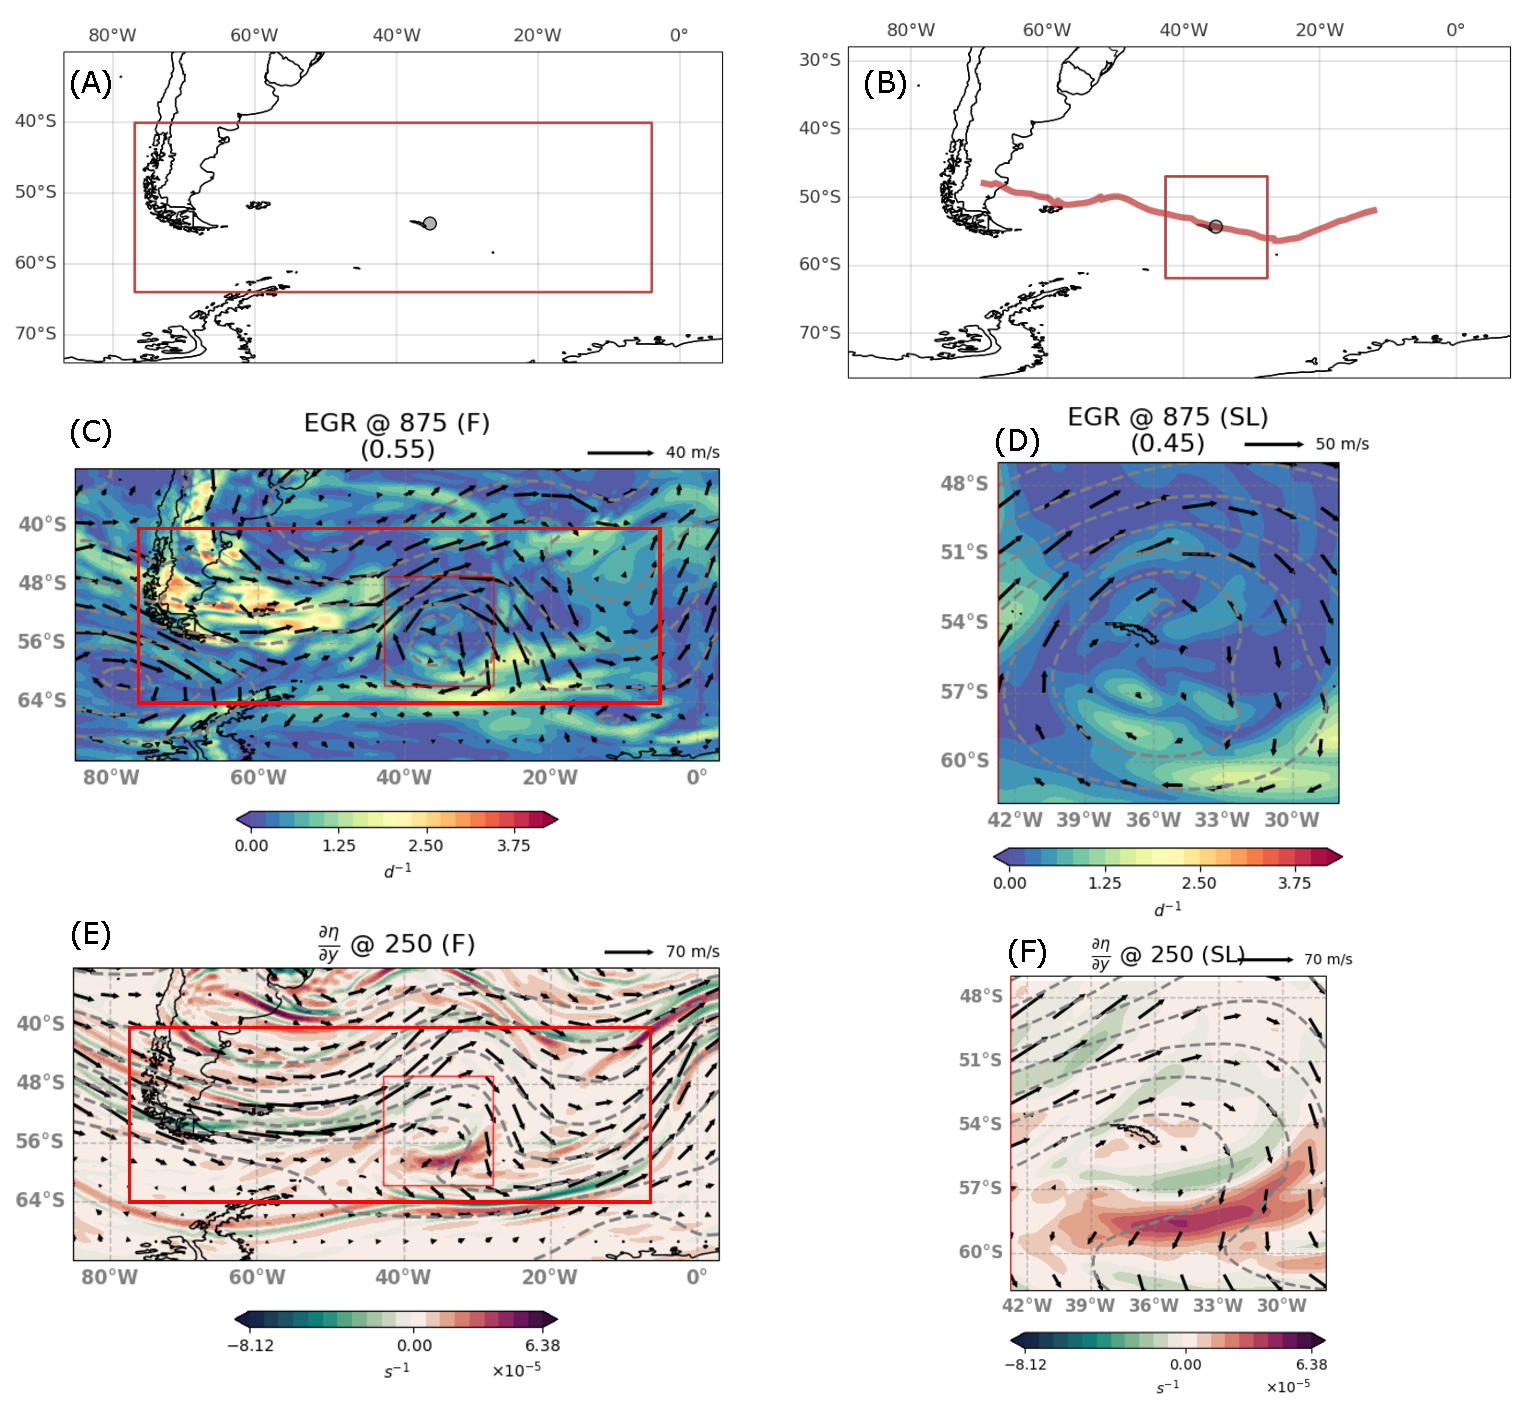
\includegraphics[width=\textwidth]{figs_6/panel_compare_fixed_sl.pdf}
    \caption[Comparative Analysis]{Comparison of barotropic and baroclinic instability analysis between the Fixed and Semi-Lagrangian Frameworks for system 19820099, during the time step of most intense $K_Z \rightarrow K_E$ conversions. (a) Computational domain for the Fixed Framework, indicated by the larger rectangle. (b) Track of the system with the Semi-Lagrangian domain, indicated by the smaller rectangle. (c) EGR fields for the Fixed domain, with the averaged EGR value in the domain shown in parentheses (0.55 $day^{-1}$). (d) EGR fields for the Semi-Lagrangian domain, with the averaged EGR value in the domain shown in parentheses (0.45 $day^{-1}$). (e) Meridional derivative of $\eta$ for the Fixed domain. (f) Meridional derivative of $\eta$ for the Semi-Lagrangian domain.}
    \label{fig:panel_compare_fixed_sl}
\end{figure}

The results presented here suggest that the Semi-Lagrangian Framework better represents the process of barotropic instability compared to the Fixed Framework. When Fixed domains are used for computing the LEC of cyclonic systems, they have to be large enough to capture the system's total displacement, which is on average approximately 5,000 km for the South Atlantic but can reach up to 10,000 km (Figure \ref{fig:pdf_total_distance}). Therefore, such domains would definitely capture the baroclinic regions in the mid-latitudes. However, barotropic conversions occur more localized in specific areas and thus can be overshadowed when analyzing larger domains using the Fixed Framework. The more localized aspect of the barotropic instability process is highlighted in \citet{grimm1995analysis}, which explores the role of the zonal variability of the upper tropospheric level jet in setting up barotropic instabilities responsible for the generation of teleconnection patterns not forced by localized vorticity sources. For the Semi-Lagrangian Framework, however, the computational domain is centered on the cyclonic system, where the barotropic conversions are well represented. Nevertheless, it was shown that the use of Fixed domains captures the energetics of regions not associated with eddy development, which could potentially lead to misleading results.


Furthermore, the use of the Fixed Framework for computing the LEC for EP1 systems demonstrated that even with this Framework, the importance of barotropic conversions is still evident. Thus, the apparent underestimation of the role of barotropic instability in extratropical cyclone development is not a methodological issue. It can be argued that either the role of barotropic conversions is more pronounced in this methodology only for the most intense systems, whose energetics might not have been analyzed previously, or that this issue might arise from the lack of studies investigating the energetics of such a large number of systems.

\section{Summary and Concluding Remarks}

This chapter presented the Lorenz Phase Space (LPS) diagrams, a visualization tool aimed at providing a diagnostic of the eddy-related energetics inspired by the \citet{hart2003cyclone} Cyclone Phase Space. This tool allows for a quick assessment of the dynamical mechanisms related to cyclone development, such as baroclinic and barotropic energy conversions, imports of both eddy kinetic and available potential energy, as well as the generation of eddy available potential energy due to diabatic processes (convective activity).

The energy cycle of all systems with genesis in the Southwestern Atlantic and Southeast America (SESA) region was dissected for each life cycle phase and then clustered using the K-means algorithm to determine their energy patterns (EP). Three EPs were found, and the differences among them were defined by their energy states. EP1 represents the most common cyclones in the SESA region, presenting low energy states and the lowest maximum relative vorticity values. Meanwhile, EPs 2 and 3 display progressively increased energy states and higher maximum vorticity values.

The identified EPs indicate the following behavior for the energy cycle of cyclones in the SESA region:

\begin{itemize}
    \item During cyclogenesis and incipient development, the systems present low baroclinic and barotropic conversions, but with imports of eddy APE. The imports of eddy kinetic energy are initially neutral, but more intense systems present progressively higher levels of imports of such energy.
    \item In the intensification phase, the baroclinic conversions and imports of eddy kinetic energy are often at their maximum, with their relative magnitude increasing from EP1 to 3. During this phase, imports of eddy APE become neutral.
    \item Both baroclinic conversions and imports of eddy kinetic energy tend to diminish in the mature phase. Meanwhile, barotropic conversions become more intense and the systems begin to export eddy APE, with progressively higher values for both terms from EPs 1 to 3.
    \item The baroclinic and barotropic conversion terms, as well as boundary fluxes of eddy APE, tend to become more neutral during the decay phase, while the export of eddy kinetic energy tends to intensify.
\end{itemize}

Significant variability in this mean behavior across different life cycle configurations or genesis regions and seasons was not found, although the overall magnitude of the terms tends to vary, with some exceptions noted.

The importance of barotropic conversions for cyclone development was not evidenced by previous studies. To determine whether barotropic instability was occurring near the cyclone systems, it was investigated if the Rayleigh-Kuo criterion was being satisfied, which was confirmed by the analysis for EP1 systems. These results were replicated using the Fixed Framework, revealing that even with a different methodology, the signal of barotropic conversions was still noted, although weakened.

Besides directly providing kinetic energy to the cyclone systems, barotropic instability might also contribute to cyclonic development via the Ekman pumping mechanism. Once the initial perturbation is established, Ekman pumping in the boundary layer can enhance vertical movements \citep[e.g.]{hamouda2019ekman}, leading to cloud formation and latent heat release. Another mechanism that might be at play is Wave-CISK \citep{lindzen1974wave,raymond1976wave}. Convergence induced by Wave-CISK can contribute to reducing low pressure, drawing in moist air, and enhancing upward motion. This process leads to increased cloud formation and latent heat release, further fueling cyclonic development.

Nevertheless, the barotropic conversion term $C_K$ is composed of five distinct terms: meridional advection of zonal momentum, meridional shear of meridional wind, interaction of eddy zonal wind with zonal meridional wind, and vertical advection of zonal momentum. Only the first three terms are strictly related to the classical view of barotropic instability \citep{rayleigh1895stability,kuo1949dynamic,holton1973introduction}. Meanwhile, the last two terms involve vertical transports of momentum, which are intimately related to the presence of vertical wind shear and, therefore, due to the thermal-wind relationship, i.e., baroclinicity. A future study will be conducted to assess which terms dominate in the barotropic conversions. The author believes this can help to better understand the dynamical processes presented here and will open avenues for further research.

In conclusion, the results shown here indicate barotropic instability as an important dynamical mechanism for cyclone development in the SESA region. The lack of previous indication of such behavior is due to either a lack of analysis of such a large dataset or due to methodological limitations, or both.

It is proposed here to use the LPS diagrams as the visual representation of the dynamic processes related to cyclone development, similarly to how \citet{hart2003cyclone} is a representation of the cyclones' thermal structure and symmetry. In Figure \ref{fig:lps_example_mixed}, LPS diagram 1 is represented along with the dynamical processes related to each of its quadrants. Cyclones in the top-right quadrant are said to be related to baroclinic instability, while in the bottom-left, barotropic instability, and in the top-left, both instabilities are occurring. Lastly, in the bottom-right, the eddy is feeding the zonal circulation.

While this research contributed to understanding the mechanisms related to each quadrant in LPS diagram 1, this is not the case for LPS diagram 2 (Figure \ref{fig:lps_example_imports}). While the imports of eddy kinetic energy have been suggested to be related to downstream development \citep{michaelides1999quasi}, this relationship was not further investigated. Also, for imports of eddy APE, from the mathematical expression for such term, it is tentative to relate it to thermal advection or heat fluxes, previously related as important mechanisms for cyclone development on SESA region \citep{gozzo2014subtropical, dutra2017structure, gramcianinov2019properties}. It is then suggested here for future research to investigate such relationships.

Nevertheless, the LPS diagrams are not yet ready to be used as a diagnostic tool for cyclone classification. For this, future research should be conducted on examining the EPs for distinct cyclonic systems, such as tropical and subtropical cyclones. It is the author's best wish to continue with this research, providing an integrated Framework for cyclone classification, alongside with \citet{hart2003cyclone} diagrams, which will account for cyclones' Material, Formal, Efficient, and Final Causes.

\begin{figure}[!htbp]
\centering
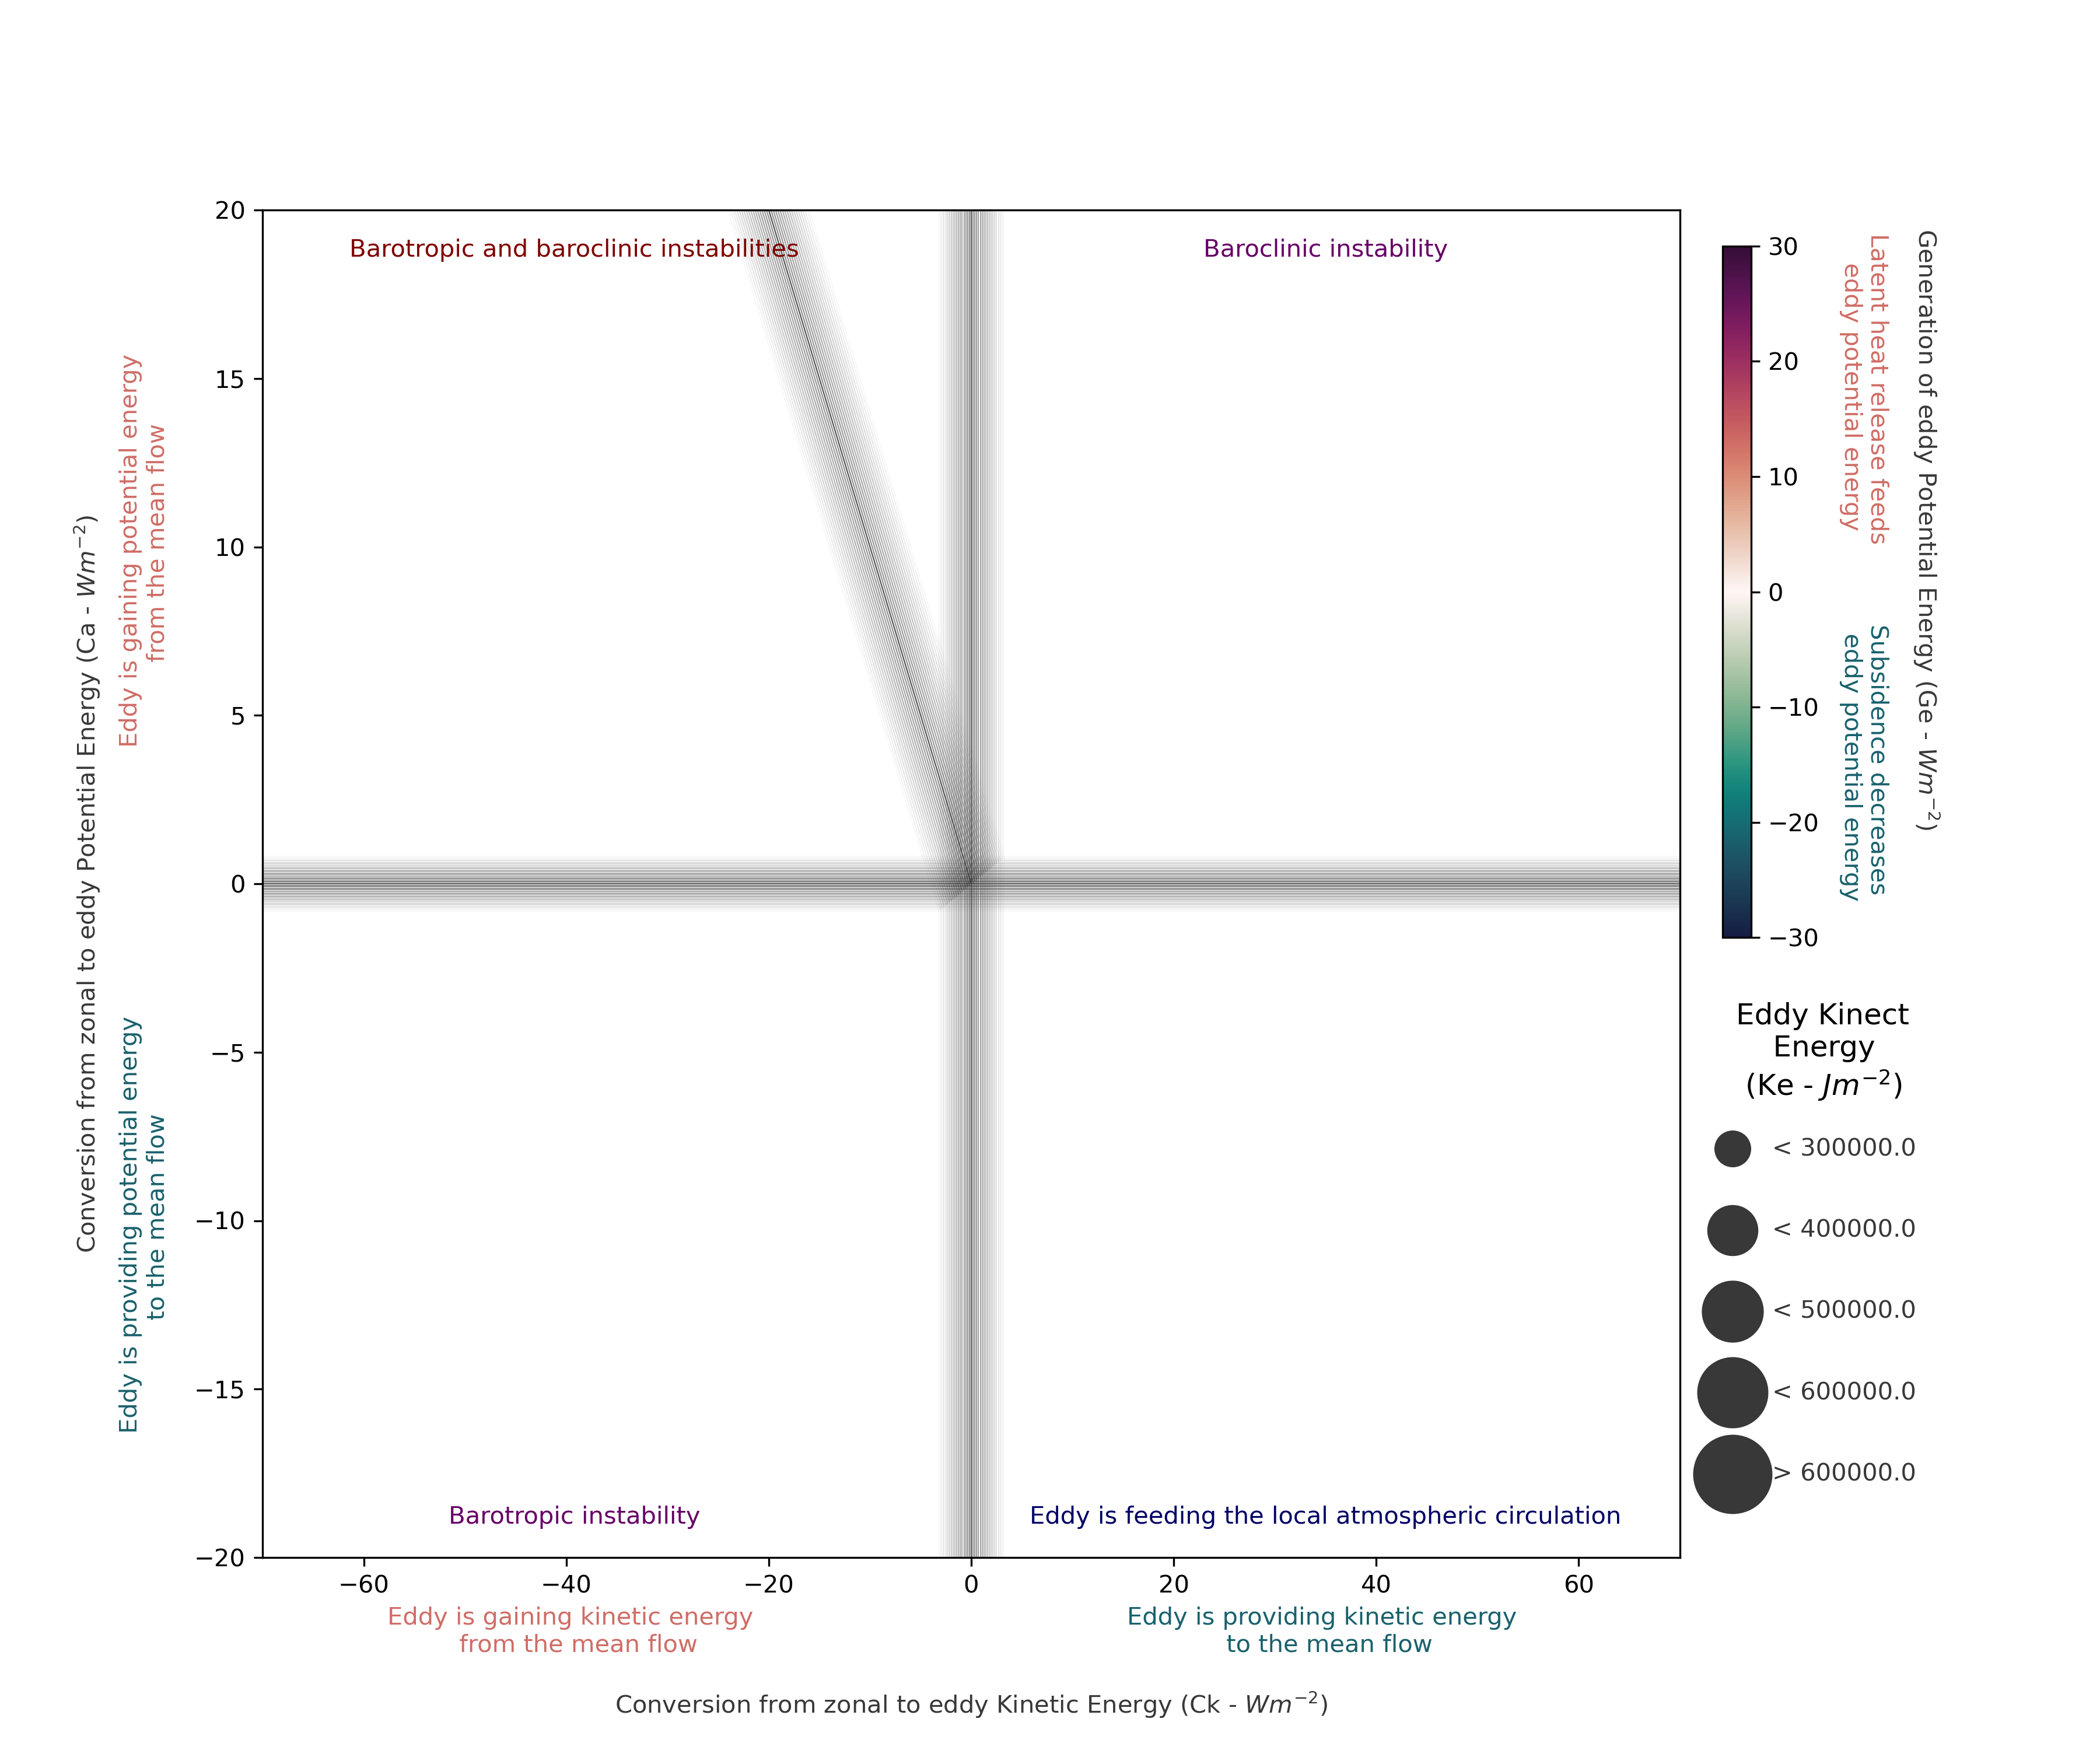
\includegraphics[width=\textwidth]{figs_6/lps_example_mixed.png}
\caption[LPS 1 - Dynamical Processes]{Lorenz Phase Space (LPS) diagram 1 representation with each dynamical process related to each quadrant represented.}
\label{fig:lps_example_mixed}
\end{figure}

\begin{figure}[!htbp]
\centering
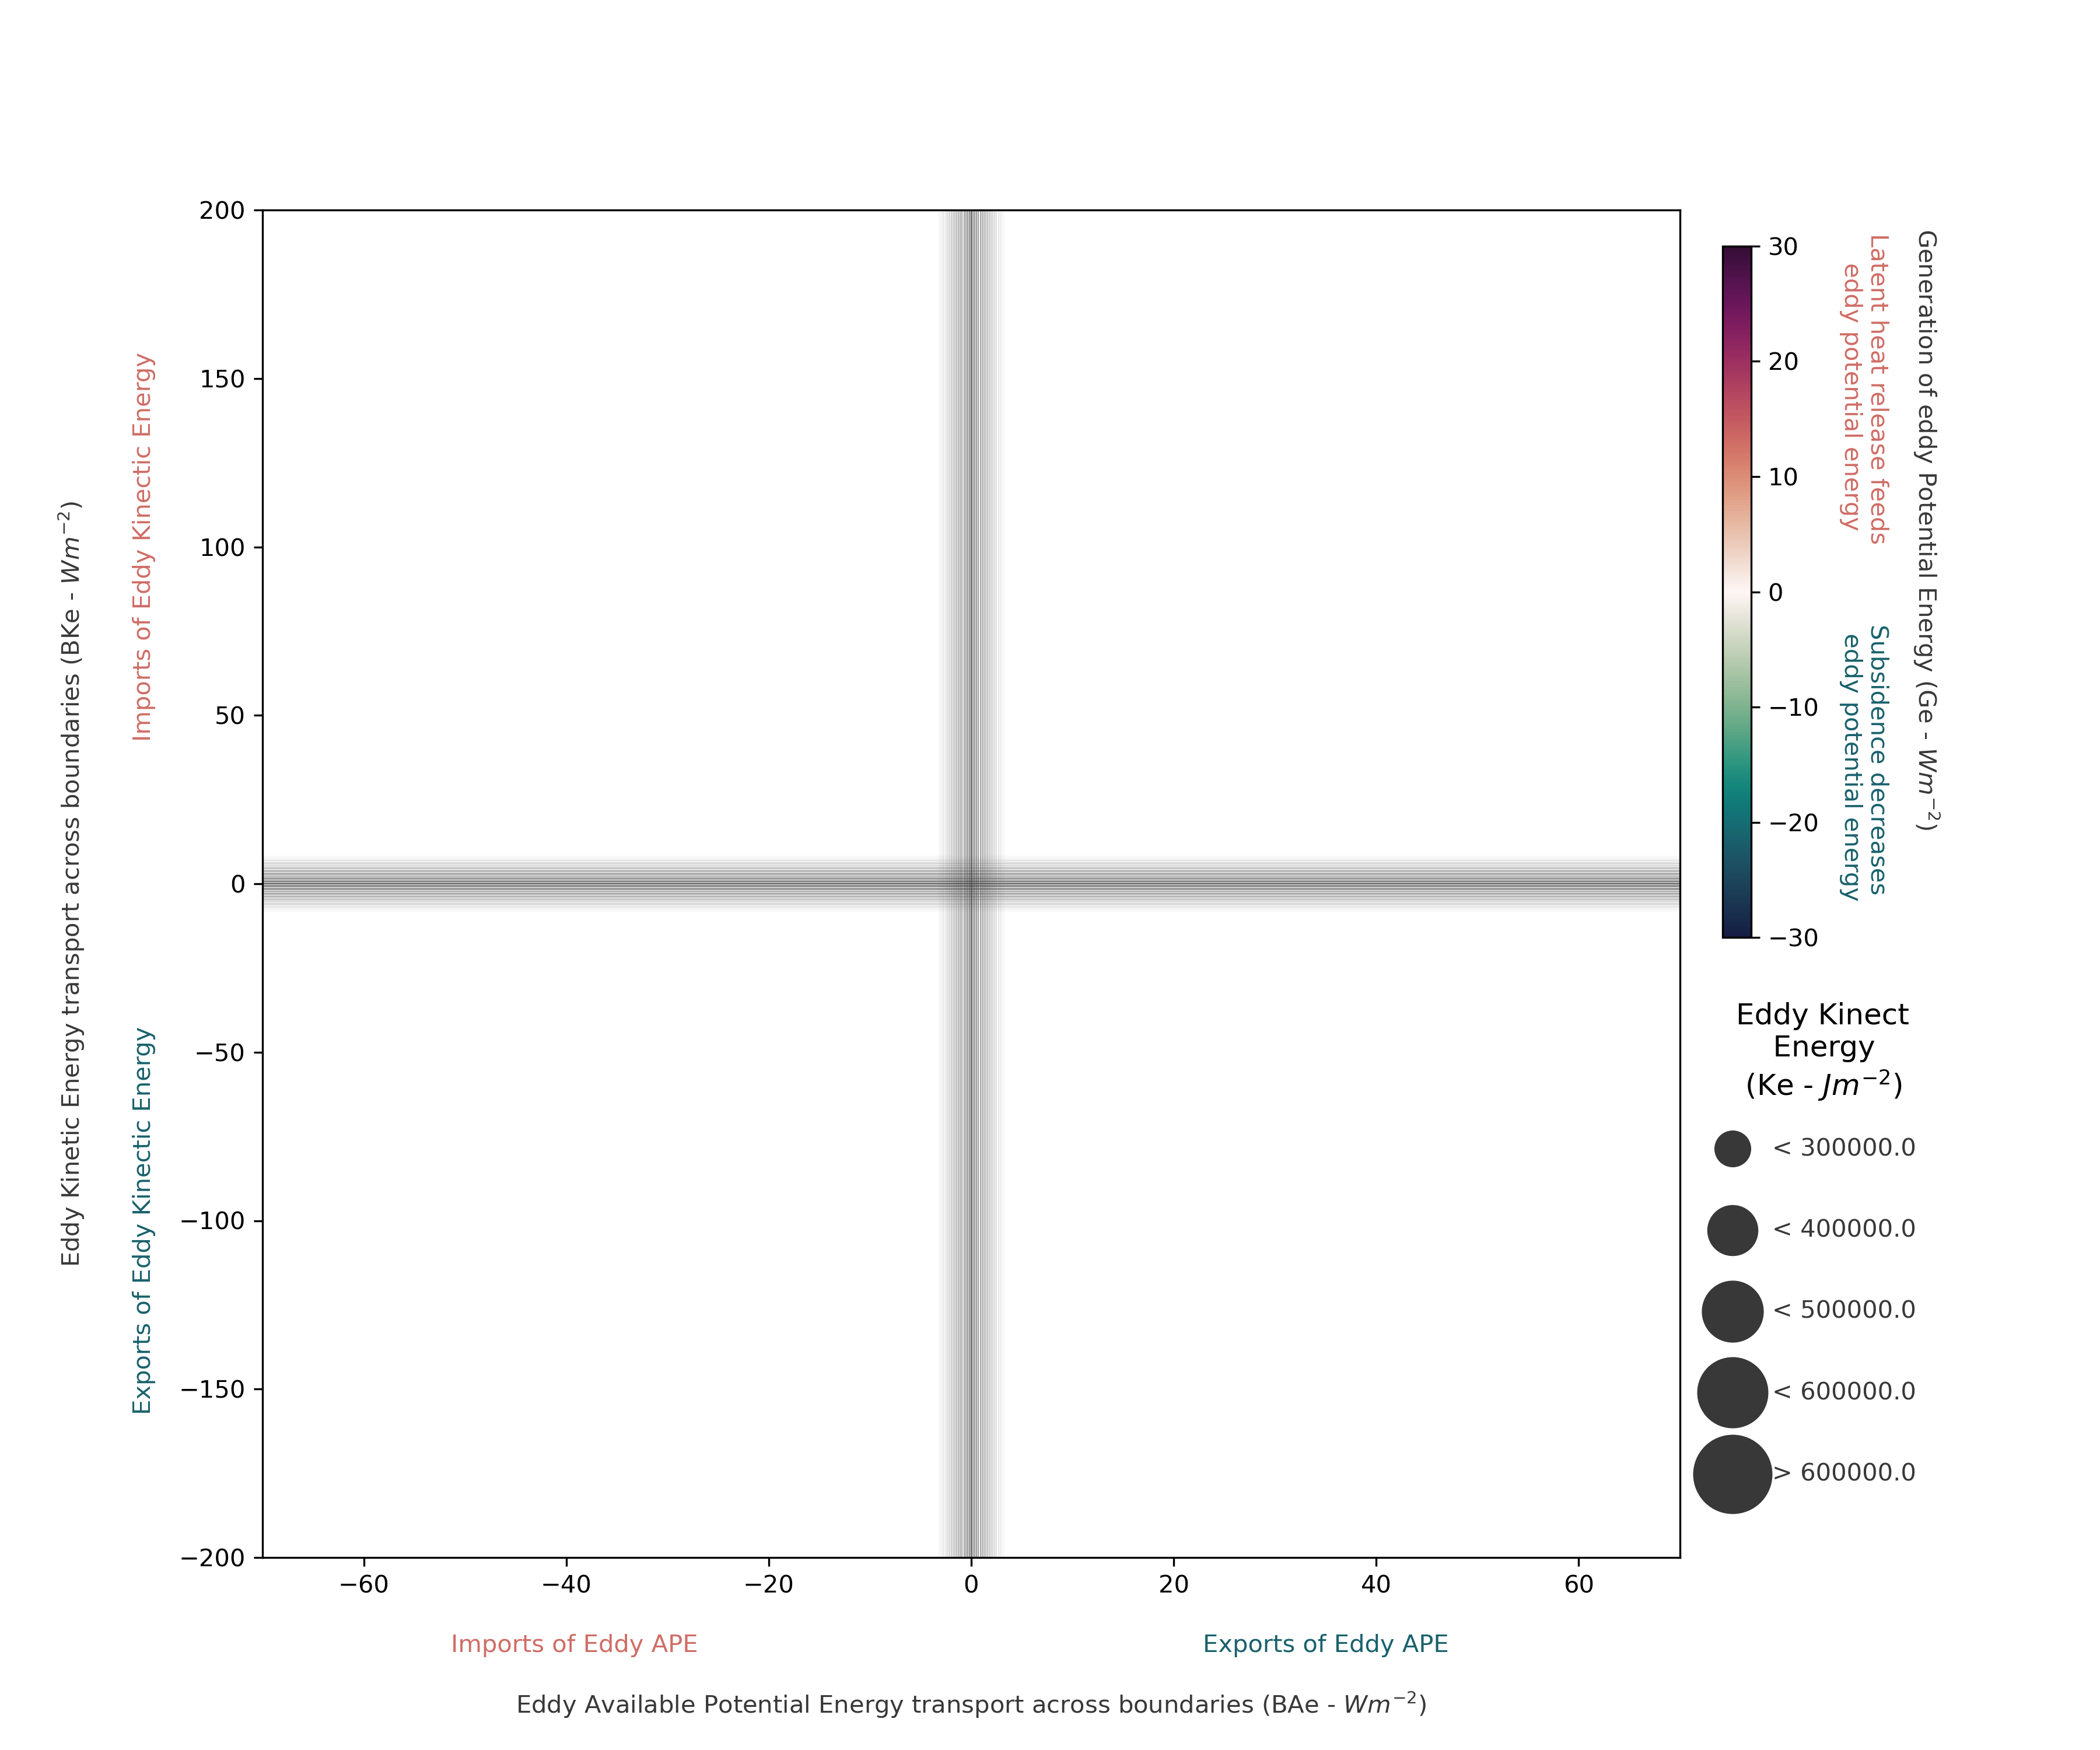
\includegraphics[width=\textwidth]{figs_6/lps_example_imports.png}
\caption[LPS 2 - Dynamical Processes]{Lorenz Phase Space (LPS) diagram 2 representation with each dynamical process related to each quadrant represented.}
\label{fig:lps_example_imports}
\end{figure}
